\documentclass[lettersize,journal]{IEEEtran}
\usepackage{amsmath,amsfonts}
\usepackage{algorithmic}
\usepackage{adjustbox}
\usepackage{algorithm}
\usepackage{array}
\usepackage{subcaption}
\usepackage{textcomp}
\usepackage{stfloats}
\usepackage{url}
\usepackage{verbatim}
\usepackage{graphicx}
\usepackage{ragged2e}
\usepackage{gensymb}
\usepackage{cite}
\usepackage{capt-of}
\usepackage{tikz}
\usetikzlibrary{arrows.meta, positioning, shadows, shapes.geometric, shapes.multipart}

\tikzstyle{startstop} = [rectangle, rounded corners, minimum width=3cm, minimum height=1.5cm,text centered, draw=black, fill=red!30]

\tikzstyle{process} = [rectangle, minimum width=3.5cm, minimum height=1cm, text centered, draw=black, fill=blue!30]
\tikzstyle{arrow} = [thick,->,>=stealth]


%\hyphenation{op-tical net-works semi-conduc-tor IEEE-Xplore}
% updated with editorial comments 8/9/2021

\begin{document}

\title{Digital Twin Buildings: 3D Modeling, GIS Integration, and Visual Descriptions Using Gaussian Splatting, ChatGPT/Deepseek, and Google Maps Platform}

\author{Kyle Gao, ~\IEEEmembership{Graduate Student Member IEEE}, Dening Lu, Liangzhi Li, Nan Chen,  Hongjie He, Linlin Xu*, \IEEEmembership{Member IEEE}, Jonathan Li, \IEEEmembership{Fellow IEEE}
% <-this % stops a space
\thanks{Manuscript received February xx, 2025; accepted xxxx xx 2025. Date of publication xxxx xx, 2025. This work was supported in part by the NSERC discovery grant under No. RGPIN-2022-03741. (Corresponding author: J. Li, junli@uwaterloo.ca and L. Xu, lincoln.xu@ucalgary.ca) }
\thanks{Kyle Gao, Dening Lu, and Jonathan Li (cross-appointed) are with the Department of Systems Design Engineering, University of Waterloo, Canada (e-mail: {y56gao, d62lu, junli}@uwaterloo.ca).}
\thanks{Hongjie He and Jonathan Li are with the Department of Geography and Environmental Management, University of Waterloo, Canada (e-mail: {h69he@uwaterloo.ca
, junli@}@uwaterloo.ca).}
\thanks{Nan Chen is with the School of Computer Science, Xi'an Aeronautical University, China (e-mail: chcdut@126.com).}
\thanks{Liangzhi Li is with the College of Land Engineering, Chang'an University, China (e-mail: liliangzhi@chd.edu.cn).}
\thanks{Linlin Xu is with the Department of Geomatics
Engineering, University of Calgary, Canada (e-mail: lincoln.xu@ucalgary.ca).}}


\markboth{}%
{Shell \MakeLowercase{\textit{et al.}}: 3DGS Diffusion}

% Remember, if you use this you must call \IEEEpubidadjcol in the second
% column for its text to clear the IEEEpubid mark.

\maketitle

\begin{abstract}
We present an image blending pipeline, \textit{IBURD}, that creates realistic synthetic images to assist in the training of deep detectors for use on underwater autonomous vehicles (AUVs) for marine debris detection tasks. 
Specifically, IBURD generates both images of underwater debris and their pixel-level annotations, using source images of debris objects, their annotations, and target background images of marine environments. 
With Poisson editing and style transfer techniques, IBURD is even able to robustly blend transparent objects into arbitrary backgrounds and automatically adjust the style of blended images using the blurriness metric of target background images. 
These generated images of marine debris in actual underwater backgrounds address the data scarcity and data variety problems faced by deep-learned vision algorithms in challenging underwater conditions, and can enable the use of AUVs for environmental cleanup missions. 
Both quantitative and robotic evaluations of IBURD demonstrate the efficacy of the proposed approach for robotic detection of marine debris. 
\end{abstract}




\begin{IEEEkeywords}
Gaussian Splatting, ChatGPT, Deepseek, Large Language Models, Multi-Agent, AI, 3D Reconstruction, Google Maps, Remote Sensing, Urban Buildings, Urban Digital Twin
\end{IEEEkeywords}


%%%%%%%%%%%%%%%%%%%%%%%%%%%%%%%%%%%%%%%%%%


%%%%%%%%%%%%%%%%%%%%%%%%%%%%%%%%%%%%%%%%%%

\IEEEPARstart{L}everaging advanced algorithms and neural network architectures like Transformers~\cite{vaswani2023attentionneed}, AI has been empowered with strong reasoning ability and made tremendous progress in recent years. Breakthroughs in model design and training methodologies have allowed machines to excel in complex tasks, including Natural Language Processing (NLP) applications such as language translation, sentiment analysis, and text generation, achieving high accuracy and fostering intuitive human-computer interactions. Similarly, advancements in Computer Vision (CV) have empowered AI to analyze and interpret images, videos, and audio sequences with remarkable precision. In healthcare, Artificial Intelligence (AI) is revolutionizing medicine by enabling data-driven insights, improving diagnostics, and personalizing treatments~\cite{topol2019,Esteva2017,KOUROU20158}. These innovations have enabled significant applications, such as medical imaging analysis, disease diagnosis, pathology, radiology workflow optimization, and surgical assistance, transforming patient care and clinical workflows~\cite{empeek2024,pmc2021}.


The medical field faces unique challenges in data interpretation and decision-making for healthcare specialists; they must analyze diverse types of information including medical imaging (X-rays, MRIs, pathology slides), clinical notes, patient histories, and real-time observations. Medical images are critical for diagnostic checks and measurements, such as identifying anatomical abnormalities, quantifying disease progression, or assessing treatment efficacy. On the other hand, textual data, such as clinical notes, nurse evaluations, and patient histories, provide essential context for screening, understanding symptoms, and documenting disease progression. Textual outputs, such as radiology reports or discharge summaries, are equally vital, as they synthesize findings into actionable insights for clinicians. The complexity and volume of this multi-modal medical data often lead to cognitive overload, impacting the speed and accuracy of diagnoses. Traditional single-modality approaches, which treat images and text separately, fail to capture the intricate relationships between visual findings and clinical context. This limitation underscores the need for integrated vision-language models (VLMs) that can bridge the gap between these modalities\cite{bordes2024introductionvisionlanguagemodeling}, enabling more comprehensive and accurate decision-making in healthcare. This integrated approach promises to enhance clinical decision-making by providing more contextually informed insights and reducing the cognitive burden on healthcare providers.

\begin{figure*}[ht]
    \centering
    \includegraphics[width=\linewidth]{images/methods2.png}
    \caption{\textbf{Comprehensive Framework for Medical Vision-Language Models (VLMs)}. \textbf{(a)} Training involves processing diverse inputs such as images, texts, metadata, and historical data, followed by pre-training. \textbf{(b)} Benchmarking is conducted on a variety of medical datasets including GMAI-MMBench, OmniMedVQA, RadBench, and others. \textbf{(c)} Advanced training strategies are employed, such as vision-text alignment, knowledge distillation, masked language modeling, contrastive learning, and parameter-efficient tuning. \textbf{(d)} Evaluation strategies encompass automated metrics like BLEU, ROUGE, BERTScore, and clinical-specific tools like CheXpert Labeler and RadGraph, alongside human evaluation. \textbf{(e)} Integration of VLMs into the medical workflow leverages contextual data to provide actionable insights and improve clinical decision-making.}
    \label{fig:method}
\end{figure*}

However, visual and language provide totally different modalities that are not trivial to be integrated directly. As illustrated in Fig.~\ref{fig:method}, existing works address this challenge through various strategies, including vision-text alignment (in MedViL\cite{devlin2019bertpretrainingdeepbidirectional}, MedCLIP\cite{radford2021learningtransferablevisualmodels}, BioMedCLIP\cite{zhang2024biomedclipmultimodalbiomedicalfoundation}, VividMed\cite{luo2024vividmedvisionlanguagemodel}), knowledge distillation with VividMed\cite{luo2024vividmedvisionlanguagemodel}, masked language modeling (in MedViL\cite{devlin2019bertpretrainingdeepbidirectional} and BioMedCLIP\cite{zhang2024biomedclipmultimodalbiomedicalfoundation}) and contrastive learning in MedCLIP\cite{radford2021learningtransferablevisualmodels}, BioViL\cite{Boecking2022} \& ConVIRT\cite{zhang2022contrastivelearningmedicalvisual}. More recent advancements have introduced additional approaches, such as frozen encoders and Q-Former (e.g., BLIP-2\cite{li2023blip2bootstrappinglanguageimagepretraining}, InstructBLIP\cite{dai2023instructblipgeneralpurposevisionlanguagemodels}), image-text pair learning and fine-tuning (e.g., LLaVA\cite{liu2023visualinstructiontuning}, LLaVA-Med\cite{li2023llavamedtraininglargelanguageandvision}, BiomedGPT\cite{Zhang2024}, MedVInT\cite{zhang2024pmcvqavisualinstructiontuning}), parameter-efficient tuning (e.g., LLaMA-Adapter-V2\cite{zhang2024llamaadapterefficientfinetuninglanguage}), two-stage training (e.g., MiniGPT-4\cite{zhu2023minigpt4enhancingvisionlanguageunderstanding}), and modular multimodal pre-training (e.g., mPLUG-Owl\cite{ye2024mplugowlmodularizationempowerslarge}, Otter\cite{li2023ottermultimodalmodelincontext}) and the Sigmoid Loss for Language-Image Pre-Training (SigLIP)\cite{zhai2023sigmoidlosslanguageimage}. SigLIP replaces traditional softmax-based contrastive learning with a simpler sigmoid loss approach, enabling more efficient and scalable training by treating image-text pair alignment as a binary classification task. These methods aim to establish coherent relationships between visual inputs and textual outputs, enabling models to effectively interpret and generate relevant information across modalities. As a comparison, the contrastive learning-based methods leverage the similarities and differences between paired visual and textual data to enhance model robustness and generalization.

This paper provides a comprehensive review of VLMs and their applications in healthcare. We first discuss how VLMs are constructed by integrating advancements in NLP and computer vision. Next, we summarize key methodologies and advancements in the field, including state-of-the-art models like Qwen-VL\cite{bai2023qwenvlversatilevisionlanguagemodel}, RadFM\cite{wu2023generalistfoundationmodelradiology}, and DeepSeek-VL\cite{lu2024deepseekvlrealworldvisionlanguageunderstanding}. We then explore how VLMs are applied in the medical domain, highlighting their potential to improve diagnostic accuracy, clinical decision-making, and other healthcare tasks. Finally, we conclude by outlining future directions and challenges in the integration of VLMs into healthcare practices.

\section{Background and Related Works}


\subsection{ChatGPT/Deepseek and API}
Large Language Models (LLMs) are neural networks, typically Transformer-based \cite{transformer}, pre-trained on extensive, diverse text/image corpora, typically sourced from web crawls. These models, designed for Natural Language Processing (NLP), typically interpret text-based prompts and generate text-based outputs. Certain models, such as "DeepseekV3/R1" and their variants \cite{deepseekv3, deepseekr1}, support object character recognition (OCR, i.e., reading text from images). Models like "ChatGPT-4o" \cite{gpt4} and its variants additionally support full interpretation and analysis of image content.

LLMs have achieved widespread adoption since 2023. Beyond basic image and text interpretation, these models recently exhibited expert-level problem-solving in various scientific and engineering domains \cite{gpqa, math500}.

Due to their large size, LLMs often face hardware constraints for local deployment. While popular LLM providers such as OpenAI and Deepseek, provide web browser interfaces for their models, they also offer Application Programming Interfaces (APIs). These APIs enable client-side software or code to query LLMs hosted on OpenAI or Deepseek servers, facilitating large-scale data processing without requiring human-in-the-loop manipulations via browser interfaces. Unlike traditional local deep learning, which necessitates GPUs for both training and inference, API-based LLM querying requires minimal local hardware and can be deloyed on devices such as mobile phones. 
\begin{table*}[ht]
\centering
\captionof{table}{TABLE OF IMPORTANT DEEPSEEK AND OPENAI LLMs}
\begin{tabular}{l|l|l|l|c|c|c}
\hline
Model Name            & Model Class          & Model Type    & Image Processing & Parameters    & \begin{tabular}[c]{@{}l@{}}API call price/1M\\ Input Tokens (USD)\end{tabular} & \begin{tabular}[c]{@{}l@{}}API call price/1M\\ Output Tokens (USD)\end{tabular} \\ \hline
chatgpt4o-latest      & GPT4o                & Autoregressive & Analysis         & $\sim$ 1000+B       & 2.5                                                                & 10                                                                \\ 
gpt-4o-mini           & GPT4o Mini          & Autoregressive & Analysis         & $\sim$10's of B        & 0.15                                                               & 0.6                                                               \\ 
deepseek-chat         & Deepseek V3          & Autoregressive & OCR               & 617B          & *0.14 $\times$ 0.1*                                                    & 1.10                                                              \\ 
deepseek-reasoner     & Deepseek R1 (V3-base) & Reasoning & OCR               & 617B          & 0.14                                                               & 2.19                                                              \\ 
\textit{gpt-o1$^{1}$}                & GPT-o1 (GPT4-base) & Reasoning     & None              & $\sim$175B        & 15                                                                 & 60                                                                \\ \hline
\end{tabular}\par
\smallskip
\justifying
\noindent
Table compiled on 2025-01-31.  OpenAI models are not open-sourced, their model sizes (parameters) are estimated (B = billions, M = millions). $^1$We did not include gpt-o1 in our experiments due to cost, but we include its specifications for comparison. *The Deepseek V3 API call input token price is discounted by 90\% if input caching is used for repeated identical prompting.* \label{Tab:models}
\end{table*}
\subsection{Google Maps Platform API}
Google Map Platform is a cloud-based mapping service and a part of Google Cloud. Its API allows the client device to connect to various cloud-based GIS, mapping, and remote sensing services hosted on the Google Cloud servers. 

The services utilized in this research include remote sensing image retrieval, map retrieval, elevation data retrieval, geocoding/reverse geocoding, and building polygon retrieval. However, Google Maps Platform also offers other APIs for urban and environmental research, including real-time traffic data, solar potential data, air quality data, and plant pollen data, in addition to the full suite of commonly used Google Maps navigation and mapping tools. 

Although less known in the remote sensing and GIS community than its sister application Google Earth Engine, Google Map Platform has been used in a variety of GIS research including navigation, object tracking, city modeling, image and map retrieval, geospatial data analysis for commercial and industrial applications \cite{maps1,maps2,maps3,maps4}. It is also used as part of many commercial software for cloud-based mapping integration. 

\subsection{Google Earth Studio}
Google Earth Studio \cite{google_earth_studio} is a web-based animation tool that leverages Google Earth's satellite imagery and 3D terrain data. The tool is especially useful for creating geospatial visualizations, as it is integrated with Google Earth’s geographic data. It allows for the retrieval of images from user-specified camera poses at user-specified locations. In this research, we use Google Earth Studio to retrieve 360 $\degree$ multi-view remote sensing images of a building from its address, postal code, place name, or geographic coordinates following \cite{gao_3dgs,gbm}.



%\vspace{0.5cm}
%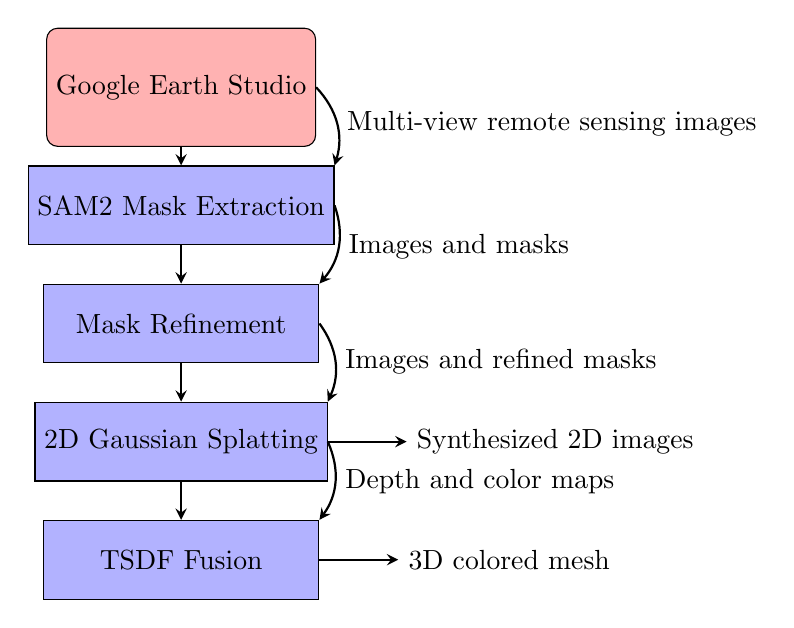
\begin{tikzpicture}[node distance=1.5cm]

% Nodes
\node (start) [startstop] {Google Earth Studio};
\node (process1) [process, below of=start] {SAM2 Mask Extraction};
\node (process2) [process, below of=process1] {Mask Refinement};
\node (process3) [process, below of=process2] {2D Gaussian Splatting};
\node (process4) [process, below of=process3] {TSDF Fusion};

% Arrows
\draw [arrow] (start) --  (process1);
\draw [arrow] (process1) -- (process2);
\draw [arrow] (process2) -- (process3);
\draw [arrow] (process3) -- (process4);
\draw [arrow, bend left] (start.east) to node[midway, right] {Multi-view remote sensing images} (process1.north east);
\draw [arrow, bend left] (process1.east) to node[midway, right] {Images and masks} (process2.north east);
\draw [arrow, bend left] (process2.east) to node[midway, right] {Images and refined masks} (process3.north east);
\draw [arrow, bend left] (process3.east) to node[midway, right] {Depth and color maps} (process4.north east);


\draw [arrow] (process3.east) -- ++(1cm,0) node[right] {Synthesized 2D images};
\draw [arrow] (process4.east) -- ++(1cm,0) node[right] {3D colored mesh};
\end{tikzpicture}
\captionof{figure}{Flowchart of GBM 3D mesh extraction. The output data modality at each step is denoted on the right. Processes and modules are boxed in blue. Figure sourced from \cite{gbm}.} \label{fig:gbmpipeline}

%\vspace{0.5cm}

%%%%%%%%%%%%%%%%%%%%%%%%%%%%%%%%%%%%%%%%%%%%
%%%%%%%%%%%%%%%%%%%%%%%%%%%%%%%%%%%%%%%%%%%%
% %%%%%%%%%%%%%%%%%%%%%%%%%%%%%%%%%%%%%%%%%%%%
% \begin{figure}[!htbp]
% \centering
% \includegraphics[width=1.0\linewidth]{Figures/EdgeMLP.png}
% \caption{(Placeholder) Mechanism of \edgemlp}
% \label{fig:edgemlp}
% \end{figure}
% %%%%%%%%%%%%%%%%%%%%%%%%%%%%%%%%%%%%%%%%%%%%
% \FloatBarrier
\section{Proposed method: \sgs}
\label{sec:Method}
% \paragraph{}
Figure~\ref{fig:sgsarchitecture} depicts our proposed method \sgs. In the following, we discuss its major components.
%\paragraph{Edge Probability Encoding Module (module I).}
\subsection{Module I: Edge Probability Encoding}
Given input $\gG$, the edge probability encoding module (\edgemlp) maps the node features to edge weights in the range $[0,1]$ followed by normalization to turn the learned weights into probabilities. The learned edge weights represent the model's unnormalized confidence in the existence of each edge. 
%However, the sum of these scores across all edges may not necessarily sum to 1. Hence, the normalization is required.
% We use a Multi-layer Perceptron to learn the probability $p(e_{uv})$ for each edge $e_{uv}\in E$. $p(e_{uv})$ represents the likelihood of sampling  edge $(u,v)$ for sparsification. 
% 
%%%%%%% sid before
% \edgemlp learns the edge weights as a function of node encodings $\vh^{(i)}_u,\vh^{(i)}_v$:
% \begin{equation*}
%     \vh_{u}^{(i)} = \relu(\Phi^{(i)}, \vh_u^{(i-1)}\oplus\mathrm{AGG}(\{\vh_{r}^{(i-1)}:r\in \gN(u)\})),
% \end{equation*}
% \begin{equation}
% \label{eq:w_uv}
% w(e_{uv}) =  \texttt{Sigmoid}(\mlp_{\phi}((\vh^{(i)}_u - \vh^{(i)}_v) \oplus (\vh^{(i)}_u \odot \vh^{(i)}_v))).
% \end{equation}
% Here, $h^{(0)}_u = \vx_u$, $\gN(u)$ denotes the set of neighbors of node $u$, $\mathrm{AGG}$ indicates the aggregation operation from \texttt{GraphSAGE}~\cite{hamilton2017inductive}, $\oplus$ indicates concatenation and $\odot$ represents elementwise multiplication.
% There are several options available for encoding \(\vh^{(i)}_u\), such as \texttt{GCN} and \mlp. Special consideration is needed when using convolutional layers for large graphs. At this stage, we can create a random sparse subgraph or draw from a prior probability distribution (eq.~\ref{eq:prior}). This subgraph will differ from the one utilized later in the downstream GNN module. 
% Additionally, among other ways, concatenating the subtraction and multiplication of two embeddings~\cite{reimers2019sentence} is very effective.
% 
%%%%%%% sid after
% \edgemlp learns the edge weights of $(u,v)$ as a function of node embeddings $\vh^{(i)}_u,\vh^{(i)}_v$:
% \begin{equation}
% \label{eq:w_uv}
% w(e_{uv}) = \sigmoid(\mlp_{\phi}((\vh^{(i)}_u - \vh^{(i)}_v) \oplus (\vh^{(i)}_u \odot \vh^{(i)}_v))).
% \end{equation}
% Here, $\sigmoid$ refers to \texttt{Sigmoid} activation function, $\oplus$ indicates concatenation, and $\odot$ represents element-wise multiplication. The embedding $\vh^{(i)}_u$ of node $u$, can be computed from \texttt{MLP} or using convolutional layers such as SAGE~\cite{hamilton2017inductive} or GCN~\cite{kipf2016semi}. For example, if \texttt{SAGE} layer is used then, 
% \begin{equation}
% \label{eq:embh_u}
%     \vh_{u}^{(i)} = \relu(\mW^{(i)}, \vh_u^{(i-1)}\oplus\mathrm{AGG}(\{\vh_{r}^{(i-1)}:r\in \gN(u)\})).
% \end{equation}
% Here, $h^{(0)}_u = \vx_u$, $\mW^{(i)}$ is the learnable weight matrix at $i$-th layer, $\gN(u)$ denotes the set of neighbors of node $u$, $\mathrm{AGG}$ indicates the aggregation operation (e.g., \texttt{mean, max}).
% 
% \textcolor{blue}{
% For large-scale graphs, the neighborhood expansion $r \in \gN(u)$ in equation~\ref{eq:embh_u} is computationally heavy on memory. Thus instead of considering all neighbors, we propose to take a subset of neighbors $\tilde{\gN}(u) \subset \gN(u)$ following a fixed prior probability distribution, $q_u(\gN(u))$. We considered two such distributions: (i) Uniform distribution:  $\forall r \in \gN(u), q_u(r) = \frac{1}{\abs{\gN(u)}}$. and (ii) Degree-proportionate distribution: $\forall r \in \gN(u), q_u(r) \propto (\frac{1}{d_u} + \frac{1}{d_r})$
% }
\edgemlp learns the edge weights of $(u,v)$ as a function of node embeddings $\vh_u,\vh_v$:
\begin{equation}
\label{eq:w_uv}
w(e_{uv}) = \sigmoid(\mlp_{\phi}((\vh_u - \vh_v) \oplus (\vh_u \odot \vh_v))).
\end{equation}
Here, $\sigmoid$ refers to \texttt{Sigmoid} activation function, $\oplus$ indicates concatenation, and $\odot$ represents element-wise multiplication. Let us assume $\vh_u$ indicates the node embedding in matrix $\mH$ corresponding to node $u$. Thus the node embedding matrix $\mH$ can be computed from an \mlp in the following manner: 
$\mH = \relu(\mlp_\mW(\mX))$, where $\mlp_\mW$ is an MLP with weights $\mW$. 
% $h_u$ indicates the node embedding in $\mH$ corresponding to node $u$. 
\mlp is computationally efficient; however, it does not exploit the graph structural information. As a result, \mlp is not necessarily the most effective choice, as we have shown later in the Ablation study (section \ref{app:ablationstudy}).

A common way to incorporate graph structural information  is to use graph convolutions such as vanilla GCN~\cite{kipf2016semi} or SAGE convolution~\cite{hamilton2017inductive}.
For instance, one can compute graph-structure aware node embedding matrix using a single-layer \texttt{GCN} as the following: $\mH = \sigma(\hat{\mA}_\gG\mX\mW)$,  where, $\mW$ is the learnable weight matrix. However, considering the entire graph $\mA_\gG$ is memory intensive for large graphs. 

Thus \sgs takes a length $\floor{\frac{q|\gE|}{100})}$ subset of edges $\gE_\mathrm{sp} \subseteq \gE$ following a fixed prior probability distribution $p_\mathrm{prior}$ and uses the induced subgraph $\gG[\gE_\mathrm{sp}]$ for computing node embedding $\mH$. In order to maintain good connectivity in $\gG[\gE_{sp}]$, the prior distribution is defined as the following:
% We have considered two such prior distributions: (i) uniform: $\forall_{(u,v) \in \gE}~p_\mathrm{prior}(u,v) = \frac{1}{\abs{\gE}}$ and (ii) degree-proportionate:
$\forall_{(u,v) \in \gE}~p_\mathrm{prior}(u,v) \propto (\frac{1}{d_u} + \frac{1}{d_v})$, where $d_u,d_v$ are the degrees of nodes $u,v$.
% 
% The sampled sparse subgraph $\gE_\mathrm{sp}$ is used for node embedding. 
% This sparse graph is different from the one used later in the downstream GNN module, which is learned.
% Sid: I think mentioning SAGE here would be overkill; GCN explains our case.
% The only purpose of this sparse subgraph is to aid the efficient computation of embeddings, which is different from the one utilized later in the downstream GNN module.

% Furthermore, among other ways, concatenating the subtraction and multiplication of two embeddings~\cite{reimers2019sentence} is very effective.

% \subsubsection{Normalization.}
%\paragraph{Normalization.}
\noindent\textbf{Normalization.} 
Normalization turns the learned edge weights into a valid probability distribution. One simple choice is \emph{sum-normalization} computed as following: $\tilde{p}(e_{uv}) = {w(e_{uv})}/{\sum_{(u,v)\in \gE} w(e_{uv})}$.
Another choice is \emph{softmax-normalization} with temperature annealing,
\begin{equation}
\label{eq:softmaxnorm}
\tilde{p}(e_{uv}) = \frac{\exp(w(e_{uv})/T)}{\sum_{(u,v)\in \gE} \exp(w(e_{uv})/T)}.
\end{equation}
Here, $T>0$ is the temperature parameter.
% that interpolates the distribution from one-hot to uniform.
% When $T$ is large, the sampling distribution becomes close to uniform, while a small value of $T$ makes the samples identical to those from the categorical distribution~\cite{jang2016categorical}. 
When $T$ is large, the learned distribution $\tilde{p}$ approaches uniform distribution over edges, whereas the learned distribution $\tilde{p}$ approaches categorical distribution when $T$ is small~\cite{jang2016categorical}. 
% 
% A high and low $T$ value corresponds to the exploration and exploitation behavior of the distribution.
As the learned distribution approaches uniform distribution, the model tends to explore more diverse subgraphs from subgraph space $\gG_q$. On the other hand, as the learned distribution approaches categorical distribution, the model tends to explore less in $\gG_q$.
Hence, we vary $T$ as a function of training iterations such that in early iterations, the algorithm explores more while narrowing down to its preferred search space later on. 
We execute such an annealing mechanism with the following equation:
%where $t$ is the temperature that varies as a function of epoch in the following manner:
\begin{equation}
T = \max (T_\mathrm{min},T_0 - \mathrm{epoch} \cdot r),
\end{equation}
% 
where $r = (T_0 - T_\mathrm{min})/{\mathrm{max\_epochs}}$ is the annealing rate, $T_\mathrm{min}$ is the minimum allowable temperature, and $T_0$ is the initial temperature. The temperature linearly decreases from the initial value $T_0$ to its final value $T_\mathrm{min}$ with the epochs. We keep track of the $T$-value that gives the best validation accuracy and use it later during inference.
 
Alg.~\ref{alg:edgmlp} shows the pseudocode for \edgemlp. 

% %%%%%%%%%%%%%%%%%%
\begin{algorithm}[!hbt]
\caption{\edgemlp Module}
\begin{algorithmic}[1] % The [1] here is for line numbering
\small
\STATE \textbf{Input:} $\gG (\gV, \gE, \mX)$, sample \% $q$, \#layers $L$, $\mathrm{epoch}$,  $\mathrm{max\_epochs}$
\STATE $\forall_{(u,v)\in\gE}~p_\mathrm{prior}(u,v) \gets \frac{1/d_u + 1/d_v}{\sum_{i,j\in \gE} (1/d_i + 1/d_j)}$
\STATE $\gE_\mathrm{sp} \gets \text{Multinomial}(\gE, p_\mathrm{prior}, \floor{\frac{q|\gE|}{100}})$ %\COMMENT{if $\gG$ is large otherwise use $\gE$}
\STATE $\mH \gets \texttt{GCN}_\mW(\gE_\mathrm{sp},\mX, L)$
\STATE $\forall_{(u,v)\in \gE}~\vw(u,v) = \sigma(\mlp_{\phi}((\vh^{(i)}_u - \vh^{(i)}_v) \oplus (\vh^{(i)}_u \odot \vh^{(i)}_v))$
\STATE $T \gets \max (T_\mathrm{min},T_0 - \mathrm{epoch} \cdot \frac{T_0 - T_\mathrm{min}}{\mathrm{max}\_\mathrm{epochs}})$
%\STATE $p(e_{uv}) = \frac{\exp(w(e_{uv}))/t)}{\sum_{(u,v)\in \gE} \exp(w(e_{uv}))/t)}: \forall (u,v) \in \gE $
\STATE $\tilde{p} \gets \mathrm{Softmax}(\vw/T)$    
\STATE \textbf{Return} $\tilde{p}, \vw$
\end{algorithmic}
\label{alg:edgmlp}
\end{algorithm}
% %%%%%%%%%%%%%%%%%%
% 
% As we will show later that, this learned probabilities $\tilde{p}$ can approximate the true unknown probabilities with arbitrarily small error due to the universal approximation property of $f_{\text{MLP},\phi}$.
% \paragraph{Theoretical analysis.} Let us assume that (i) there is an idealized learning ORACLE that knows the true probability distribution over the edges, (ii) the true distribution $p^*$ is a continuous function of node features $\mX$ and (iii) $\mX$ is a compact subset (bounded and closed) of Euclidean space $\mathbb{R}^n$.
% Now, the Universal Approximation Theorem states that a feed-forward neural network with at least one hidden layer and a finite number of neurons can approximate any continuous function $f: \mathbb{R}^n \rightarrow \mathbb{R}$ on a compact subset of $\mathbb{R}^n$, given a suitable choice of weights and activation functions. We use this result to state the following proposition under the assumptions I-III.
% \begin{proposition} For any error $\epsilon>0$, there exists an \mlp $f_{\mlp,\phi} = \tilde{p}$ that approximates the function $p^*$.
% \begin{equation}
% \label{eq:uapp}
% \sup_{e \in \mathcal{E}} \|\tilde{p}(\vx_e) - p^*(\vx_e)\|_1 \leq \epsilon
% \end{equation}
% where both $\tilde{p}$ and $p^*$ are functions of edge features $\vx_e = \vx_e =  (\vh^{(i)}_u - \vh^{(i)}_v | \vh^{(i)}_u \odot \vh^{(i)}_v)$ as used in equation~\ref{eq:w_uv}.
% \end{proposition}

% More discussion on this result can be found in Appendix~\ref{theo:uap}.

%\paragraph{Sparse subgraph sampling (module II).}
\subsection{Module II: Sparse Subgraph Sampling}
Given the learned distribution $\tilde{p}$ over the edges of the input graph, sparse subgraph sampling aims to construct a sparse graph with the user-given sparsity constraint $q$. We do not know which discrete distribution has $\tilde{p}$ as parameters. A natural choice is to construct $\tilde{\gG} = (\gV,\tilde{\gE},\mX)$ by assuming that $\tilde{p}$ is a parameter of a \emph{Multinomial} distribution. Hence we can sample $k=\floor{\frac{q|\gE|}{100}}$ edges as
$\tilde{\gE} \sim \text{Multinomial}(\tilde{p},k)$.

We can also construct $\tilde{\gG}$ by assuming that $\tilde{p}$ is a parameter of some categorical distribution and use \emph{Gumbel Softmax trick}~\cite{jang2016categorical}. The idea is to induce \emph{Gumbel noise} $g_{uv}\sim Gumbel(0,1)$ to the edges and select Top-$K$ edges with the highest probabilities.
% the $k$ edges using $\texttt{TopK}$ function. 
In order to sample edges according to categorical distribution, we replace our softmax-normalization (Equation~\ref{eq:softmaxnorm}) with the following:
\begin{equation}
\tilde{p}(e_{uv}) = \frac{\exp(({\log w(e_{uv})+g_{uv}})/{T})}{\sum_{(u,v)\in \gE} \exp({(\log w(e_{uv})+g_{uv})}/{T
})}.    
\end{equation}
Adding noise ensures that we are taking different samples at each time, and with low temperatures ($T=0.1, T=0.5$), the samples become identical to samples from a categorical distribution~\cite{jang2016categorical}. 
%We can also select the top-$\floor{\frac{q|\gE|}{100}}$ edges with the highest probabilities but lack exploration capability during training. However, it can give us one of the best sparse subgraphs during inference. 
%\naheed{@Sid, Discuss how we sampled from the categorical distribution with noise using Gumbel-softmax trick.}
%Sid: resource: https://docs.google.com/document/d/1HrslfnxNP6dso6DX9OXFvXSzQYF9Q-mz/edit
%We have empirically evaluated the effect of these distribution choices on the performance of \sgs in the section on ablation studies.

%\paragraph{Theoretical analysis.}
\noindent\textbf{Theoretical analysis I.} 
Let $\mathcal{E}^*$ and $\mathcal{\tilde{E}}$ denote the ordered collection of edges sampled by the idealized learning ORACLE according to true distribution $p^*$ and by \sgs according to learned probability $\tilde{p}$ respectively. For analytical convenience, let us assume that the algorithm samples $k$ edges with replacement. We have the following theorem that lower-bounds the \#edges common between sampled subgraphs from \sgs and idealized learning ORACLE.

\begin{theorem}[Lower-bound] The expected number of edges sampled by both \sgs and idealized learning ORACLE satisfies
\vspace{-10pt}
\begin{equation} 
\mathbb{E}[|\mathcal{E}^* \cap \mathcal{\tilde{E}}|] \geq k \sum_{j=1}^{|\mathcal{E}|} \frac{(p^*_j + \tilde{p}_j - \epsilon)^2}{4},
\end{equation}
where $k = \floor{q|\mathcal{E}|/100}$ with $0 \leq q \leq 100$ as a user-specified parameter and $\epsilon\in [0,1]$ is the error.
\end{theorem}
The proof is in Appendix~\ref{theo:commonedges}. The implications are:
\begin{enumerate}[wide, labelwidth=!, labelindent=2pt,itemsep=1pt,topsep=1pt]
    \item Let the true distribution be uniform. In the best-case scenario $\epsilon \rightarrow 0$ and $\tilde{p} = p^* = \frac{1}{|\mathcal{E}|}$. Then there are at least $\frac{k}{|\mathcal{E}|}$ common edges between $\tilde{\gG}$ and $\gG^*$. 
    % However, since $k < \abs{\mathcal{E}}$, the lower-bound of $\mathbb{E}[|\mathcal{E}^* \cap \mathcal{\tilde{E}}|] \geq \frac{k}{|\mathcal{E}|}$ is not very useful even though the learned distribution is accurate. 
    Since $k << \abs{\mathcal{E}}$, this specific scenario suggests that the learned sparse subgraph may not overlap much with the true one even after we have learned the true distribution. When the true distribution is uniform, every subgraph from $\gG_q$ is a global minimizer of the task-specific loss $\mathcal{L}_{CE}$. Otherwise, the learning ORACLE would have put more mass on certain edges and the distribution $p^*$ would not have been uniform. As individual subgraphs are indistinguishable in terms of performance, this case beats the purpose of supervised sparsification.

    \item Let the true distribution be one-hot. In other words, suppose $\tilde{p} = p^* = \delta_{ij}$, where $\delta_{ij}$ is the \emph{Kronecker-delta}. In this case, as $\epsilon \rightarrow 0$, the lower bound reduces to 
    \vspace{-8pt}
    \begin{equation*}
    \mathbb{E}[|\mathcal{E}^* \cap \mathcal{\tilde{E}}|] \geq k \sum_{j=1}^{|\mathcal{E}|} (\tilde{p}_j)^2 = k.
    \end{equation*}
    % \vspace{-4pt}
    This identity suggests that the sampled edges are expected to completely overlap with the true sparse subgraph. 
    
\end{enumerate}

% In practice, it would be surprising if the true distribution is uniform. If it was, the loss landscape would have been flat. 
For strong heterophilic graphs ($\gH_n$ is small), the true distribution is less likely to be uniform. Because a uniform edge sample would retain a similar node homophily as in the input graph, and such a subgraph would not be able to minimize $\mathcal{L}_{CE}$~\cite{das2024ags}. Thus, it is important for the learned probability distribution to approximate $p^*$ so that the sampled subgraph is close enough to the true one.
 
We have analyzed $\tilde{\gG}$ generated by \sgs on a synthetic graph in Appendix~\ref{app:toymoon}.

\begin{comment}
\begin{theorem}[Upper-bound] The expected number of edges sampled by both \sgs and idealized learning ORACLE satisfies
\begin{equation}
\mathbb{E}[|\mathcal{E}^* \cap \mathcal{\tilde{E}}|] \leq k (1 - \frac{\|p^* - \tilde{p}\|_1}{2}) 
\end{equation}
where $k = \floor{q|\mathcal{E}|/100}$ with $0 \leq q \leq 100$ as a user-specified parameter.
\end{theorem}

\textit{The implication of the upper bound.} When $\tilde{p} \rightarrow p^*$, the norm $\|p^* - \tilde{p}\|_1 \rightarrow 0$; therefore, the number of common edges could be close to $k$.

\end{comment}

%\paragraph{GNN module (module III).}
\subsection{Module III: Downstream GNN and Loss Functions}
At this stage, we input the sampled subgraph to a downstream GNN that supports edge weights as computed in Equation~\ref{eq:w_uv}; since the edge weights of the sampled edges are one of the ways we optimize \edgemlp via backpropagation. An example \gnn would be 
\begin{equation}
\hat{\mY} = \texttt{Softmax}(f_{\gnn,\theta}(\gV, \tilde{\gE}, \mX, \tilde{\vw})),
\end{equation}
where $\tilde{\gE}$ refers to the edges of the sampled sparse subgraph $\gG'$ and $\tilde{\vw} = \vw[\tilde{\gE}]$ contains the edge weights. 
%One of the ways gradient optimizers update the parameters of \edgemlp is by backpropagating through these sampled weights.

% We do not explicitly construct the sparse adjacency matrix $A_{\tilde{G}}$

%\paragraph{Loss functions.}
\noindent\textbf{Loss functions.} 
We introduce two regularizers to engrain various inductive biases to \sgs and combined these functions with the Cross-Entropy loss $\gL_\mathrm{CE}$ as follows:
\begin{equation}
\mathcal{L} = \alpha_1\mathcal{L}_\mathrm{CE} + \alpha_2 \mathcal{L}_\mathrm{assor} + \alpha_3 \mathcal{L}_\mathrm{cons},
\end{equation}
where $0 \leq \alpha_1,\alpha_2,\alpha_3 \leq 1$ are regularizer coefficients.

The \textbf{Assortativity loss} $\mathcal{L}_\mathrm{assor}$ uses the labels of the training nodes to force nodes with similar labels to have higher edge weights while forcing dissimilarly labeled nodes to have a small nonzero weight. This regularizer encourages edge homophily in the sampled sparse graph.
\vspace{-7pt}
\begin{equation}
\small
     \mathcal{L}_\mathrm{assor} \triangleq -\sum_{(u,v) \in \gE:u \land \gV_L \land v \in \gV_L} \mathbb{I}(y_u=y_v)\cdot \log w(e_{uv}),
\end{equation}
% \vspace{-20pt}
where $\mathbb{I}(.)$ is an indicator function that returns $0$ or $1$. 

The \textbf{Consistency loss} defined below encourages learned edge probabilities to reflect the similarity between node embeddings or features:
\vspace{-8pt}
\begin{equation}
\mathcal{L}_\mathrm{cons} \triangleq \sum_{(u,v) \in \tilde{\gE}} \|w(e_{uv}) - \mathrm{cosine}(\vh_u^l,\vh_v^l)\|,
\end{equation}
where $\mathrm{cosine}(\vh_u^l,\vh_v^l) = {\vh_u^l\cdot \vh_v^l}/{\|\vh_u^l\|\|\vh_v^l\|}$ is the cosine similarity of the learned GNN embeddings $\vh_u^l,\vh_v^l$ of nodes $u$, $v$ from layer $l$, and $w(e_{uv})$ is the learned probability for edge $(u,v)$ in the sparse graph $\tilde{\gG}$. This mechanism aligns the edge probabilities with the global graph structure and ensures that the sparsifier learns to preserve edges consistent with the broader graph relationships. 
% In ablation studies, we have evaluated the utility of these additional regularizing functions.
% 
% The dashed arrows in Fig.~\ref{fig:sgsarchitecture} illustrate the pathways of \edgemlp and \gnn model parameter updates through these losses during backpropagation. 
%Alg.~\ref{alg:sgstraining} in Appendix~\ref{app:algorithm} shows the pseudocode of our base training algorithm.
%These loss functions allow backpropagation to update \edgemlp, using only the training edges with $\gL_\mathrm{assor}$, and all the edges with $\gL_\mathrm{cons}$.


%\paragraph{Theoretical analysis.}
\noindent\textbf{Theoretical analysis II.} 
We consider vanilla GCN as a downstream GNN to examine how the sparse subgraph, $\tilde{\gG}$ from \sgs, affects node embeddings compared to the ideal subgraph $\gG^*$ from a learning ORACLE. Suppose an $L$-layer GCN produces embeddings $\tmH^{(L)}$ and $\mH^{*(L)}$ when taking $\tilde{\gG}$ and $\gG^*$ as input, respectively.
%Our goal is to analyze the respective encodings produced by a $L$-layer GCN when the input subgraphs are $\gG^*$ and , respectively. 
%$\gG^*$ (corresponding to adjacency matrix $\mA_{\gG^*}$) and $\tilde{\gG}$ (corresponding to adjacency matrix $\mA_{\tilde{\gG}}$) respectively. 
% For simplicity, we will denote the ideal and our sampled sparse matrices, $\mA_{\gG^*}$ as $\mA^*$ and $\mA_{\tilde{\gG}}$ as $\tmA$ respectively.
% 
% From eq.~\ref{eq:gcnlayer}, a single GCN layer is defined as $\mH^{(l+1)} =\sigma(\hat{\mA}\mH^{(l)}\mW^{(l)})$,
% % where $\hat{\mA} = \mD^{-1/2}\mA\mD^{-1/2}$ is the normalized adjacency matrix, $\mH^{(l)}$ is the input to the $l$-th layer with $\mH^{(0)} = \mX$, $\mW^{(l)}$ is the learnable weight matrix for $l$-th layer and $\sigma$ is non-linear activation function. 
% and an $L$-layer GCN produces embeddings $\tmH^{(L)}$ and $\mH^{*(L)}$ when it takes sparse matrices $\tmA$ and $\mA^*$ as input. 
% 
Is there an upper bound of the difference in the downstream node encodings $\mathbb{E}[\normLtwo{\tmH^{(L)} - \mH^{*(L)}}]$, due to the use of a learned subgraph?

To that end, we assume for all $l\in L$, $\normLtwo{\mW} \leq \alpha < 1$ where $\alpha$ is a constant. This is reasonable since each $\mW^{(l)}$ is typically controlled during training using regularization techniques, e.g., weight decay. As input features in $\mX$ are bounded, we also assume that there exists a constant $\beta$ such that $\forall l>0$, $\normLtwo{\mH}^{(l)} \leq \beta$. We also assume that $\sigma$ is \textit{Lipschitz continuous} with \textit{Lipschitz constant} $L_\sigma$. 
% For instance,  activation functions such as \relu, \texttt{Sigmoid}, or \texttt{TanH} are \textit{Lipschitz continuous}. 
% In particular, 
We assume \relu activation to simplify our analysis since \relu has a Lipschitz constant $L_\sigma = 1$. Under these assumptions, we have the following theorem (proof in Appendix~\ref{theo:gcnembed}). 

\begin{theorem}[Error in GCN encodings]
For sufficiently deep L-layer GCN, the error in node embeddings  

\vspace{-15pt}
{\scriptsize
\[
\mathbb{E}[\lim_{L \to \infty} \normLtwo{\tmH^{(L)} - \mH^{*(L)}}] < \frac{\beta}{1-\alpha}\sqrt{2k (1 - \sum_{j=1}^{|\mathcal{E}|} \frac{(p^*_j + \tilde{p}_j - \epsilon)^2}{4})}.
\]
}
\vspace{-15pt}
\end{theorem}
% The proof is given in Appendix~\ref{theo:gcnembed}.
 % 
% 
\subsection{\sgs Training and Additional Details}
\label{subsec:largescale}
\begin{algorithm}[!ht]
\caption{\sgs Training}
\begin{algorithmic}[1] % The [1] here is for line numbering
\small
\STATE \textbf{Input:} $\gG (\gV, \gE, \mX)$, sample \% $q$, \#layers $L$, METIS Parts $n$
% \STATE \textbf{Output:} \texttt{EdgeMLP}, \texttt{GNN}
\STATE $p_\mathrm{prior}(u,v) \gets \frac{1/d_u + 1/d_v}{\sum_{i,j\in \gE} (1/d_i + 1/d_j)}$

\STATE $\gG_\mathrm{parts} \gets \{\gG_1,\gG_2,\cdots,\gG_n\}= \mathrm{METIS} (\gG(\gV,\gE, p_\mathrm{prior}), n)$

\FOR{$\mathrm{epoch}$ in $\mathrm{max\_epochs}$}

    \FOR {$\gG_i(\gV_i,\gE_i,\mX_i,p^i_\mathrm{prior}) \in \gG_\mathrm{parts}$}
        \STATE $\tilde{p}, \vw \gets \edgemlp(\gE_i, \mX_i, L)$ \COMMENT{\textbf{Algorithm~\ref{alg:edgmlp}}}    
        \STATE $\tilde{p}_a \gets \lambda \tilde{p}+(1-\lambda)p^i_\mathrm{prior}$/*\textbf{Augmenting $\tilde{p}$ with prior}*/
        \STATE $\tilde{\gE}, \tilde{\vw} \gets \mathrm{Sample}(\tilde{p}_a, \vw, \floor{\frac{q|\gE|}{100}})$   \COMMENT{\textbf{Module II}}
        \STATE $\hat{\mY}, \tilde{\mH} \gets \mathrm{GNN}_\theta(\tilde{\gE},\mX_i,\tilde{\vw})$ \COMMENT{\textbf{Module III}}

        \STATE Compute $\gL_{CE}, \gL_\mathrm{assor}$, and $\gL_\mathrm{cons}$ using $\hat{\mY},\tilde{\mH}$
        
        \STATE $\gL \gets \alpha_1\cdot \gL_\mathrm{CE}+ \alpha_2\cdot \gL_\mathrm{assor}+ \alpha_3\cdot \gL_\mathrm{cons}$
        % 
        \STATE Backward Propagate through $\gL$
        % 
    \ENDFOR
    
\ENDFOR
%\STATE \textbf{Return} \texttt{EdgeMLP}, \texttt{GNN} 
\end{algorithmic}
\label{alg:sgstraining}
\end{algorithm}

Alg.~\ref{alg:sgstraining} outlines the pseudocode for training \sgs. \sgs starts with two precomputation steps:
i) computing the degree-proportionate edge weight as a \emph{prior} to enhance the learned distribution $\tilde{p}$ (line 1), and
ii) partitioning the input graph using METIS~\cite{karypis1997metis} for batch processing (line 2). Towards computing the loss for every partition at each iteration,  \sgs executes Edge probability encoding, Learned distribution augmentation with a prior, Sparse subgraph sampling and node embedding via GNN. Finally, the loss is backpropagated, the update pathways of which have been illustrated in Figure~\ref{fig:sgsarchitecture} earlier.

\textbf{Batch processing.} 
We can use \edgemlp from Alg.~\ref{alg:edgmlp} to compute edge weights in large-scale graphs, but efficient batch processing on edges is necessary for stochastic training of GNNs so as to reduce the risk of getting stuck in local minima.
It is crucial to select a batch of edges that have high locality, preferably from within a cluster, and we utilize METIS to achieve this. We could have made partitions small enough to fit GPUs and then applying GNN without any sparsification, similar to ClusterGCN~\cite{chiang2019cluster}. However, certain edges, such as task-irrelevant edges, may negatively impact performance, particularly in heterophilic or noisy graphs. In such cases, a high-quality learned sparse subgraph performs better than full graph, as validated in our experiments (\S\ref{subsubsec:fixedsampler}). 
% Sparsification also enables larger partitions without significant information loss.

\textbf{Augmenting $\tilde{p}$ with prior.} 
% We begin training for each graph partition by learning the probability distribution and edge weights from \edgemlp (line 5). 
While $\tilde{p}$ can be directly used to sample sparse subgraphs, the resulting subgraph may be suboptimal for message passing due to missing bridge edges connecting low-degree node pairs.
Thus augmenting the sampler with  $p_\mathrm{prior}$, which favors such edges, results in better quality sparse subgraph. $p_\mathrm{prior}$ is defined as
% Although \emph{effective resistance} can be an option, it is impractical for large graphs. 
\vspace{-8pt}
\begin{equation}
\label{eq:prior}
 p_\mathrm{prior}(u,v) \triangleq \frac{1/d_u + 1/d_v}{\sum_{i,j\in \gE} (1/d_i + 1/d_j)},
\end{equation}
where $d_u,d_v$ are degrees of nodes $u,v$. We control the emphasis of prior on the learned distribution with a parameter $\lambda \in [0,1]$, resulting in the \emph{augmented probability distribution}: $\tilde{p}_{a}(u,v) = \lambda \tilde{p}(u,v) + (1-\lambda) p_\mathrm{prior}(u,v)$ (line 7). The impact of $p_\mathrm{prior}$ on \sgs is discussed in Appendix~\ref{app:parameters}.

Another enhancement we consider is the \textbf{conditional updates} to \edgemlp. Since backpropagation is computationally expensive, we only update \edgemlp when the training F1-score from the learned sparse subgraph exceeds the baseline subgraph from $p_\mathrm{prior}$. The detailed algorithm for \sgs with conditional updates is in Appendix~\ref{app:algorithm}.

During inference, we use the learned probability distribution from \edgemlp, sample an ensemble of sparse subgraphs, and mean-aggregate their representations to produce final prediction on a test node. The pseudocode for inference (Alg.~\ref{alg:sgsinference}) is in Appendix~\ref{app:algorithm}.

\begin{comment}%\paragraph{Degree bias augmentation with a learned probability distribution.}
\noindent\textbf{Degree bias augmentation with a prior.} 
The search space for learning algorithms to identify optimal sparse graphs can be extensive in large-scale graphs. To address this, we can use a prior probability distribution $p_\mathrm{prior}$ based on \emph{degree}~\cite{zeng2019graphsaint}. This distribution favors edges connected to vertices with low degrees and assigns lower selection probabilities to edges within denser clusters. Due to computational efficiency, we chose degree-proportionate prior over \emph{effective resistance}. We control the bias between the learned and prior probability distributions using the control parameter $\lambda \in [0,1]$. The probability distribution becomes, $\tilde{p}(u,v) = \lambda \tilde{p}(u,v) + (1-\lambda) p_\mathrm{prior}(u,v)$, where $\tilde{p}$ is the learned probability distribution and degree norm $p_\mathrm{prior}$ for edge ($u,v$) is,
\vspace{-8pt}
 \begin{equation}
\label{eq:prior}
 p_\mathrm{prior}(u,v) = \frac{1/d_u + 1/d_v}{\sum_{i,j\in \gE} (1/d_i + 1/d_j)}.
\end{equation}
%\vspace{8pt}
% \vspace{-10pt}
% Alg.~\ref{alg:sgstraining} outlines the pseudocode of \sgs.

\noindent\textbf{METIS graph partitioning.}
We can use \edgemlp from Alg.~\ref{alg:edgmlp} for edge weight computation in large graphs. However, we want efficient batch processing on edges, avoid gradient accumulation, and make the training process stochastic. This helps train GNN models with fewer epochs by reducing the likelihood of getting stuck in local minima.
One crucial step is selecting a batch of edges such that the vertices in a batch of edges have high locality and preferably from within a cluster. To achieve this, we consider very fast graph partitioning methods like METIS~\cite{karypis1997metis}.

For inference, we use the probability distribution from \edgemlp, sample multiple sparse subgraphs, and aggregate their predictions. The pseudocode of inference (Alg.~\ref{alg:sgsinference}) is provided in Appendix~\ref{app:algorithm} for brevity.
\end{comment}


% \paragraph{Dynamic temperature annealing.}
% \[
% t = \max (t_\mathrm{min},t_0 - \mathrm{epoch} \cdot r)
% \]
% where $r = \frac{(t_0 - t_\mathrm{min})}{\mathrm{total}\_\mathrm{epochs}}$ is the annealing rate, $t_\mathrm{min}$ is minimum allowable temperature, and $t_0$ is the initial temperature. 
% \paragraph{Consistency loss.}

% \[
% L_\mathrm{cons} = \sum_{(u,v) \in \tilde{\gG}} \|\tilde{p}(e_{uv}) - \mathrm{cosine}(\vh_u,\vh_v)\|
% \]
% where $\mathrm{cosine}(\vh_u,\vh_v) = \frac{\vh_u\cdot \vh_v}{\|\vh_u\|\|\vh_v\|}$ is the cosine similarity of the learned GNN embeddings $\vh_u,\vh_v$ corresponding to nodes $u$ and $v$ and $p(e_{uv})$ is the learned probability for edge $(u,v)$ in the sparse graph $\tilde{\gG}$.

% \paragraph{Performance-Gated Training.}
% %%%%%%%%%%%%%%%%%%

% \noindent\textbf{Conditional update of \edgemlp.}
% Backward propagation is often the most computationally intensive part of training, so we employ a conditional mechanism to update \edgemlp selectively. We evaluate the learned sparse subgraph against a subgraph from the prior probability distribution $p_\mathrm{prior}$. If the training F1-score from the learned sparse subgraph is better than the baseline, parameters of \edgemlp are updated; otherwise, the update is skipped. Detailed algorithm for \sgs with conditional updates (Alg.~\ref{alg:sgstrainingpriorfull}) is provided in Appendix~\ref{app:algorithm}.

% \subsection{Theoretical results}
% \label{subsec:theory}
% The final objective of our theoretical analysis is to obtain an upper bound on the learned node embedding produced by module III (section 4.4.4). To obtain this upper bound we consider as a reference an idealized learning ORACLE that knows the true sampling probability distribution. Toward our final theoretical goal, first, we obtain an upper bound on the learned probability distribution (section 4.4.1). Afterwards, we obtain an upper bound on the number of common edges (section 4.4.2) which helps us bound the error in the learned Adjacency matrix (section 4.4.3). Finally, in section 4.4.4, we obtain an upper bound on the learned node embedding produced by \sgs.


% \subsection{Computational Complexity}
\textbf{Computational Complexity.}
Suppose the number of hidden dimension $H\approx F$, where $F$ is the dimension of the node features. The cost of an $L$-layer GCN is $\bigO(L(|\gE|\cdot H + |\gV| \cdot H^2))$~\cite{chiang2019cluster}. 
The cost of Alg~\ref{alg:edgmlp} is $\bigO(L(|\gE_\mathrm{sp}|\cdot H + |\gV| \cdot H^2)+ \abs{\gE}\cdot H^2)$, since computing node-embedding (line 4, Alg.~\ref{alg:edgmlp}) using sparse graph $\gE_\mathrm{sp}$ costs $\bigO(L(|\gE_\mathrm{sp}|\cdot H + |\gV| \cdot H^2))$, and edge weight computation using \mlp (line 5, Alg.~\ref{alg:edgmlp}) costs $\bigO(\abs{\gE}\cdot H^2)$. 
% 
With an $L$-layer GCN used as downstream GNN acting on the sparse subgraph $\tilde{\gE}$, the downstream GNN costs $\bigO(L(|\tilde{\gE}|\cdot H + |\gV| \cdot H^2)$. 
% For loss, $L_\mathrm{assor}$, $L_\mathrm{cons}$ is $\bigO(|\tilde{\gE}$ and $\bigO(|\tilde{\gE}|\cdot H)$ respectively. 
Since, $\abs{\gE_\mathrm{sp}}=\abs{\tilde{\gE}}$ the total complexity of \sgs  (Alg.~\ref{alg:sgstraining}) is $\bigO(L(|\tilde{\gE}|\cdot H + |\gV| \cdot H^2)+ \abs{\gE}\cdot H^2)$.

\textbf{Space complexity.} Let $n$ partitions from METIS have similar sizes. The memory requirement for \sgs with $L$-layer GCN is  $\bigO\left(\frac{|\gE| + |\gV|\cdot H}{n} + L \cdot H^2 \right)$. 
% The former part is for graph-related information, and the latter is for learnable parameters.



% $\bigO(L \cdot H^2)$ for edge weight, 
% There is a precomputation cost of $\bigO(|\gE|)$ for $p_\mathrm{prior}$, and for large-scale graphs, there is an additional one-time partition cost from METIS.

% Then computation complexity of \edgemlp 

% If $H\approx F$, then the overall complexity of $L$ layer GCN can be approximated as $\bigO(L(|\gE|\cdot H + |\gV| \cdot H^2))$. If GCN is used at \edgemlp and \gnn, then the complexity of the computation using a sparse graph of size $|\tilde{\gE}|=\floor{\frac{q|\gE|}{100}}$ becomes $\bigO(L(|\tilde{\gE}| \cdot H + |\gV| \cdot H^2)$. The cost of \mlp for the edge weight computation is $\bigO(\abs{\gE}\cdot H^2)$. There is a pre-computation cost of $\bigO(|\gE|)$ for $p_\mathrm{prior}$, and for large-scale graphs, there is an additional one-time partition cost from METIS.
% Memory requirements:
% sid: maybe remove this or put this into appendix
% The memory requirements for considering the entire graph include several components: $\bigO(|\gE|)$ for edges, $\bigO(|\gV| \cdot F)$ for features, $\bigO(L|\gV| \cdot H)$ for the hidden state, $\bigO(L \cdot H^2)$ for trainable parameters, and $\bigO(L \cdot \gV \cdot H)$ for activations and gradients. If a partitioning method like METIS is employed, resulting in $n$ partitions, each partition will require approximately $\bigO\left((|\gE| + |\gV| F + L \cdot |\gV| \cdot H)/{n}\right) + \bigO(L \cdot H^2)$ of memory.
% \begin{table*}[!tbh]
\centering
\resizebox{\textwidth}{!}{%
\begin{tabular}{clcccccccccc}
\toprule
\multicolumn{1}{l}{} &  & \multicolumn{3}{c}{\textbf{CLINC}} & \multicolumn{3}{c}{\textbf{BANKING}} & \multicolumn{3}{c}{\textbf{StackOverflow}} & \multicolumn{1}{l}{} \\ \midrule
\multicolumn{1}{c|}{\textbf{KCR}} & \multicolumn{1}{l|}{\textbf{Methods}} & \textbf{ACC} & \textbf{ARI} & \multicolumn{1}{c|}{\textbf{NMI}} & \textbf{ACC} & \textbf{ARI} & \multicolumn{1}{c|}{\textbf{NMI}} & \textbf{ACC} & \textbf{ARI} & \multicolumn{1}{c|}{\textbf{NMI}} & \textbf{Average} \\ \midrule
\multicolumn{1}{c|}{} & \multicolumn{1}{l|}{GCD (CVPR 2022)} & 83.29 & 76.77 & \multicolumn{1}{c|}{93.22} & 21.17 & 9.35 & \multicolumn{1}{c|}{43.41} & 17.00 & 3.42 & \multicolumn{1}{c|}{14.57} & 40.24 \\
\multicolumn{1}{c|}{} & \multicolumn{1}{l|}{SimGCD (ICCV 2023)} & 83.24 & 75.89 & \multicolumn{1}{c|}{92.79} & 25.62 & 12.67 & \multicolumn{1}{c|}{47.46} & 18.50 & 6.49 & \multicolumn{1}{c|}{17.91} & 42.29 \\
\multicolumn{1}{c|}{} & \multicolumn{1}{l|}{Loop (ACL 2024)} & 84.89 & 77.43 & \multicolumn{1}{c|}{93.26} & 21.56 & 10.24 & \multicolumn{1}{c|}{44.77} & 18.80 & 5.76 & \multicolumn{1}{c|}{17.54} & 41.58 \\
\multicolumn{1}{c|}{\multirow{-4}{*}{5\%}} & \multicolumn{1}{l|}{\cellcolor{blue!18}\textbf{\MethodName (Ours)}} & \cellcolor{blue!18}\textbf{88.18} & \cellcolor{blue!18}\textbf{82.40} & \multicolumn{1}{c|}{\cellcolor{blue!18}\textbf{94.94}} & \cellcolor{blue!18}\textbf{30.94} & \cellcolor{blue!18}\textbf{18.32} & \multicolumn{1}{c|}{\cellcolor{blue!18}\textbf{54.05}} & \cellcolor{blue!18}\textbf{22.30} & \cellcolor{blue!18}\textbf{8.32} & \multicolumn{1}{c|}{\cellcolor{blue!18}\textbf{21.25}} & \cellcolor{blue!18}\textbf{46.74} \\ \midrule
\multicolumn{1}{c|}{} & \multicolumn{1}{l|}{GCD (CVPR 2022)} & 82.04 & 75.95 & \multicolumn{1}{c|}{93.33} & 59.09 & 46.34 & \multicolumn{1}{c|}{76.22} & 75.40 & 56.01 & \multicolumn{1}{c|}{72.66} & 70.78 \\
\multicolumn{1}{c|}{} & \multicolumn{1}{l|}{SimGCD (ICCV 2023)} & 84.71 & 77.08 & \multicolumn{1}{c|}{93.27} & 60.03 & 47.80 & \multicolumn{1}{c|}{76.53} & 77.10 & 57.70 & \multicolumn{1}{c|}{72.30} & 71.84 \\
\multicolumn{1}{c|}{} & \multicolumn{1}{l|}{Loop (ACL 2024)} & 84.89 & 78.12 & \multicolumn{1}{c|}{93.52} & 64.97 & 53.05 & \multicolumn{1}{c|}{79.14} & 80.50 & \textbf{62.97} & \multicolumn{1}{c|}{75.98} & 74.79 \\
\multicolumn{1}{c|}{\multirow{-4}{*}{10\%}} & \multicolumn{1}{l|}{\cellcolor{blue!18}\textbf{\MethodName (Ours)}} & \cellcolor{blue!18}\textbf{88.71} & \cellcolor{blue!18}\textbf{83.29} & \multicolumn{1}{c|}{\cellcolor{blue!18}\textbf{95.21}} & \cellcolor{blue!18}\textbf{67.99} & \cellcolor{blue!18}\textbf{57.30} & \multicolumn{1}{c|}{\cellcolor{blue!18}\textbf{82.23}} & \cellcolor{blue!18}\textbf{82.40} & \cellcolor{blue!18}62.81 & \multicolumn{1}{c|}{\cellcolor{blue!18}\textbf{79.67}} & \cellcolor{blue!18}\textbf{77.73} \\ 
\midrule
\multicolumn{1}{c|}{} & \multicolumn{1}{l|}{DeepAligned (AAAI 2021)} & 74.07 & 64.63 & \multicolumn{1}{c|}{88.97} & 49.08 & 37.62 & \multicolumn{1}{c|}{70.50} & 54.50 & 37.96 & \multicolumn{1}{c|}{50.86} & 58.69 \\
\multicolumn{1}{c|}{} & \multicolumn{1}{l|}{MTP-CLNN (ACL 2022)} & 83.26 & 76.20 & \multicolumn{1}{c|}{93.17} & 65.06 & 52.91 & \multicolumn{1}{c|}{80.04} & 74.70 & 54.80 & \multicolumn{1}{c|}{73.35} & 72.61 \\
\multicolumn{1}{c|}{} & \multicolumn{1}{l|}{GCD (CVPR 2022)} & 82.31 & 75.45 & \multicolumn{1}{c|}{92.94} & 69.64 & 58.30 & \multicolumn{1}{c|}{82.17} & 81.60 & 65.90 & \multicolumn{1}{c|}{78.76} & 76.34 \\
\multicolumn{1}{c|}{} & \multicolumn{1}{l|}{ProbNID (ACL 2023)} & 71.56 & 63.25 & \multicolumn{1}{c|}{89.21} & 55.75 & 44.25 & \multicolumn{1}{c|}{74.37} & 54.10 & 38.10 & \multicolumn{1}{c|}{53.70} & 60.48 \\
\multicolumn{1}{c|}{} & \multicolumn{1}{l|}{USNID (TKDE 2023)} & 83.12 & 77.95 & \multicolumn{1}{c|}{94.17} & 65.85 & 56.53 & \multicolumn{1}{c|}{81.94} & 75.76 & 65.45 & \multicolumn{1}{c|}{74.91} & 75.08 \\
\multicolumn{1}{c|}{} & \multicolumn{1}{l|}{SimGCD (ICCV 2023)} & 84.44 & 77.53 & \multicolumn{1}{c|}{93.44} & 69.55 & 57.86 & \multicolumn{1}{c|}{81.71} & 79.80 & 65.19 & \multicolumn{1}{c|}{79.09} & 76.51 \\
\multicolumn{1}{c|}{} & \multicolumn{1}{l|}{CsePL (EMNLP 2023)} & 86.16 & 79.65 & \multicolumn{1}{c|}{94.07} & 71.06 & 60.36 & \multicolumn{1}{c|}{83.22} & 79.47 & 64.92 & \multicolumn{1}{c|}{74.88} & 77.09 \\
\multicolumn{1}{c|}{} & \multicolumn{1}{l|}{ALUP (NAACL 2024)} & 88.40 & 82.44 & \multicolumn{1}{c|}{94.84} & 74.61 & 62.64 & \multicolumn{1}{c|}{84.06} & 82.20 & 64.54 & \multicolumn{1}{c|}{76.58} & 78.92 \\
\multicolumn{1}{c|}{} & \multicolumn{1}{l|}{Loop (ACL 2024)} & 86.58 & 80.67 & \multicolumn{1}{c|}{94.38} & 71.40 & 60.95 & \multicolumn{1}{c|}{83.37} & 82.20 & 66.29 & \multicolumn{1}{c|}{79.10} & 78.33 \\
\multicolumn{1}{c|}{\multirow{-10}{*}{25\%}} & \multicolumn{1}{l|}{\cellcolor{blue!18}\textbf{\MethodName (Ours)}} & \cellcolor{blue!18}\textbf{91.51} & \cellcolor{blue!18}\textbf{87.07} & \multicolumn{1}{c|}{\cellcolor{blue!18}\textbf{96.27}} & \cellcolor{blue!18}\textbf{76.98} & \cellcolor{blue!18}\textbf{66.00} & \multicolumn{1}{c|}{\cellcolor{blue!18}\textbf{85.62}} & \cellcolor{blue!18}\textbf{84.10} & \cellcolor{blue!18}\textbf{71.01} & \multicolumn{1}{c|}{\cellcolor{blue!18}\textbf{80.90}} & \cellcolor{blue!18}\textbf{82.16} \\ 

\midrule

\multicolumn{1}{c|}{} & \multicolumn{1}{l|}{DeepAligned (AAAI 2021)} & 80.70 & 72.56 & \multicolumn{1}{c|}{91.59} & 59.38 & 47.95 & \multicolumn{1}{c|}{76.67} & 74.52 & 57.62 & \multicolumn{1}{c|}{68.28} & 69.92 \\
\multicolumn{1}{c|}{} & \multicolumn{1}{l|}{MTP-CLNN (ACL 2022)} & 86.18 & 80.17 & \multicolumn{1}{c|}{94.30} & 70.97 & 60.17 & \multicolumn{1}{c|}{83.42} & 80.36 & 62.24 & \multicolumn{1}{c|}{76.66} & 77.16 \\
\multicolumn{1}{c|}{} & \multicolumn{1}{l|}{GCD (CVPR 2022)} & 86.53 & 81.06 & \multicolumn{1}{c|}{94.60} & 74.42 & 63.83 & \multicolumn{1}{c|}{84.84} & 85.60 & 72.20 & \multicolumn{1}{c|}{80.12} & 80.36 \\
\multicolumn{1}{c|}{} & \multicolumn{1}{l|}{ProbNID (ACL 2023)} & 82.62 & 75.27 & \multicolumn{1}{c|}{92.72} & 63.02 & 50.42 & \multicolumn{1}{c|}{77.95} & 73.20 & 62.46 & \multicolumn{1}{c|}{74.54} & 72.47 \\
\multicolumn{1}{c|}{} & \multicolumn{1}{l|}{USNID (TKDE 2023)} & 87.22 & 82.87 & \multicolumn{1}{c|}{95.45} & 73.27 & 63.77 & \multicolumn{1}{c|}{85.05} & 82.06 & 71.63 & \multicolumn{1}{c|}{78.77} & 80.01 \\
\multicolumn{1}{c|}{} & \multicolumn{1}{l|}{SimGCD (ICCV 2023)} & 87.24 & 81.65 & \multicolumn{1}{c|}{94.83} & 74.42 & 64.17 & \multicolumn{1}{c|}{85.08} & 82.00 & 70.67 & \multicolumn{1}{c|}{80.44} & 80.06 \\
\multicolumn{1}{c|}{} & \multicolumn{1}{l|}{CsePL (EMNLP 2023)} & 88.66 & 83.14 & \multicolumn{1}{c|}{95.09} & 76.94 & 66.66 & \multicolumn{1}{c|}{85.65} & 85.68 & 71.99 & \multicolumn{1}{c|}{80.28} & 81.57 \\
\multicolumn{1}{c|}{} & \multicolumn{1}{l|}{ALUP (NAACL 2024)} & 90.53 & 84.84 & \multicolumn{1}{c|}{95.97} & 79.45 & 68.78 & \multicolumn{1}{c|}{86.79} & 86.70 & 73.85 & \multicolumn{1}{c|}{81.45} & 83.15 \\
\multicolumn{1}{c|}{} & \multicolumn{1}{l|}{Loop (ACL 2024)} & 90.98 & 85.15 & \multicolumn{1}{c|}{95.59} & 75.06 & 65.70 & \multicolumn{1}{c|}{85.43} & 85.90 & 72.45 & \multicolumn{1}{c|}{80.56} & 81.87 \\
\multicolumn{1}{c|}{\multirow{-10}{*}{50\%}} & \multicolumn{1}{l|}{\cellcolor{blue!18}\textbf{\MethodName (Ours)}} & \cellcolor{blue!18}\textbf{94.53} & \cellcolor{blue!18}\textbf{90.79} & \multicolumn{1}{c|}{\cellcolor{blue!18}\textbf{97.12}} & \cellcolor{blue!18}\textbf{80.26} & \cellcolor{blue!18}\textbf{70.40} & \multicolumn{1}{c|}{\cellcolor{blue!18}\textbf{87.65}} & \cellcolor{blue!18}\textbf{89.40} & \cellcolor{blue!18}\textbf{78.92} & \multicolumn{1}{c|}{\cellcolor{blue!18}\textbf{85.04}} & \cellcolor{blue!18}\textbf{86.01} \\ 

\bottomrule
\end{tabular}%
}
% \caption{Main results.}
\caption{Main results of \MethodName compared to baseline methods across different datasets and known category ratios (KCR). \MethodName outperforms both standard GCD approaches and the latest LLM-based work Loop \cite{an-etal-2024-generalized}, showing significant improvements especially on the challenging BANKING dataset and with limited known categories. Performance gains are observed across most KCRs, metrics, and datasets.}
\label{tab:main_result}
\end{table*}
% \input{figure/token_len_and_task}

We now present the experimental results on Spec-Bench, along with an in-depth analysis of HD.

\subsection{Main Result}

Table~\ref{tab:main} presents our main results, averaged across all cases of Spec-Bench using three models, at both low temperature (\(T=0.0\)) and high temperature (\(T=1.0\)). First, our proposed method, HD, achieves the outperforming acceleration gain across all scenarios. In detail, when temperature is 0.0, HD achieves over 1.5x faster inference speed compared to autoregressive decoding, whereas the other methods fail to exceed a 1.4x speedup. Also, while the acceleration gain at \(T=1.0\) is slightly lower than \(T=0.0\), HD still achieves the fastest inference speed compared to all other methods across all models. These results demonstrate that our hierarchical framework effectively enhances inference speed by incorporating diverse token sources into three databases organized by temporal locality.

\begin{figure*}[t!]
\centering
\begin{minipage}{0.34\textwidth}
    \centering
    \includegraphics[width=0.99\textwidth]{figure/access_database.jpg}
\end{minipage}
\hfill
\begin{minipage}{0.65\textwidth}
    \centering
    \includegraphics[width=0.99\textwidth]{figure/task_pattern.jpg}
\end{minipage}
\vspace{-1.2em}
\caption{\small (Left) Verify success and draft latency for the databases $\mathcal{D}_c$, $\mathcal{D}_m$, and $\mathcal{D}_s$ in HD. Verify success represents the proportion of accepted accesses relative to the total accesses. (Right) Verify success density plots for each database across six tasks in Spec-Bench. Both results are conducted on Spec-Bench by using Llama-2-7b.}
\label{fig:access_database_and_task_pattern}
\vspace{-1.2em}
\end{figure*}


Beyond acceleration gains, we analyze the additional latency caused by the drafting process, which adds overhead that is absent in autoregressive decoding, and also evaluate how accurately the drafting step retrieves tokens that align with the LLM’s output. 
Regarding drafting latency, LADE requires an extremely short time—under 0.01 ms per draft—whereas REST takes significantly longer, with latency close to 3.00 ms. 
However, drafting accuracy shows the opposite trend: LADE exhibits lower values for both the acceptance ratio (\(\alpha\)) and mean accepted tokens (\(\tau\)), while REST achieves higher values for both. 
Notably, our proposed method, HD, drafts slightly faster than REST, even though accessing the same extensive database, and accurately predicts 70\% of generated tokens, achieving the highest accuracy among all other methods. 
These results indicate that HD successfully balances increased accuracy with reduced drafting latency through hierarchical database access, resulting in significant acceleration gain.

\paragraph{Comparison with Non-Database Methods} 
We compare diverse database drafting methods with two non-database drafting methods, SpS~\cite{SpS} and MEDUSA~\cite{MEDUSA}, to confirm whether the performance is competitive without additional training. 
As shown in Figure~\ref{fig:temperature_and_task}, while other database drafting methods significantly underperform compared to non-database drafting methods, our proposed method, HD, outperforms SpS and substantially narrows the performance gaps with MEDUSA. 
This demonstrates that our proposed method shows the potential to achieve more significant acceleration gain without retraining the models by exploiting data resources common in real-world serving scenarios.

\paragraph{Robustness across Tasks} 
We evaluate the robustness of database drafting methods across various generation tasks, as illustrated on the right side of Figure~\ref{fig:temperature_and_task}. 
Relying on a single source results in variability in acceleration gains, causing most methods, except HD, to show inconsistent performance with concave regions in specific tasks. 
Specifically, PLD achieves significant acceleration in tasks like Summarization and RAG but offers minimal improvements in Translation and QA. 
Additionally, other methods exhibit varying acceleration gains depending on the model used—REST, for example, performs well with Llama-7b in summarization but shows weaker results with Vicuna-7b, nearly matching autoregressive decoding speeds. 
In contrast, our proposed method consistently achieves the highest acceleration across all tasks and models, occupying the largest area in each plot. This demonstrates that incorporating diverse sources enhances robustness, making database drafting methods more suitable for real-world scenarios.


\subsection{Analysis}

In this subsection, we provide an in-depth analysis of HD for investigating its effectiveness.

\paragraph{Analysis of Three Databases}
The left side of Figure~\ref{fig:access_database_and_task_pattern} depicts each database's verify success ratio and draft latency. 
The verify success ratio measures the proportion of accepted cases relative to total database accesses during the verifying step.
$\mathcal{D}_c$ achieves the highest verify success ratio over 30\% with the lowest draft latency, demonstrating its effectiveness in fetching context-relevant future tokens. However, $\mathcal{D}_m$ shows a lower verify success rate, 15.5\%, with slightly higher latency, indicating that while it performs decently, it is less aligned with specific contexts. $\mathcal{D}_s$ exhibits the lowest verify success rate under 10\% and the highest draft latency over 10ms due to its larger scale and lower locality. These highlight that draft tokens with higher locality are more frequently accepted, indicating alignment with our design objectives.


\paragraph{Access Pattern across Tasks}
We analyze how our proposed method, HD, achieves consistent acceleration gain across tasks with verify success ratio of databases for each task.
As shown in the right side of Figure~\ref{fig:access_database_and_task_pattern}, $\mathcal{D}_c$ excels in tasks such as Multi-turn Conversation or Summarization, where the context-specific tokens are highly repeated, leading to high verification success. However, for tasks like translation and QA, which offer fewer explicit cues from previous inputs or contexts, $\mathcal{D}_c$ achieves lower verification success. 
In these cases, $\mathcal{D}_m$ and $\mathcal{D}_s$ compensate for the weaknesses of $\mathcal{D}_c$ by showing higher verification success compared to other tasks where $\mathcal{D}_c$ outperforms.
These results highlight how our HD efficiently accesses the appropriate database for each task, effectively leveraging the distinct strengths of diverse sources.


\paragraph{Database Access Order}
We analyze the impact of access order within the hierarchical framework, as shown in Figure~\ref{fig:order}. 
As expected, our original access order ($cms$), which prioritizes databases from highest to lowest temporal locality, achieves the highest acceptance ratio and lowest draft latency. 
While other orders maintain an acceptance ratio above 50\%, sufficient for some acceleration gain, their actual speedup is significantly lower due to additional drafting latency, reaching up to 12ms for orders like $scm$ or $smc$.
These results demonstrate that hierarchical access fully leverages the potential of multiple databases with minimal drafting latency compared to other orders, underscoring the importance of temporal locality in drafting order.

We provide additional analysis in Appendix~\ref{app:additional_result}.
\section{Conclusion}\label{sec:conclusion}

%%% Summarize main points and give brief overview of results %%%
Model-based approaches for time series classification can be effectively utilized when a model of the underlying dynamical process is available~\cite{shen2017classification}. 
Using structural identifiability (SI) analysis, structurally identifiable parameter combinations of the dynamical model can be obtained. 
Individual time series observations may then be represented as point estimates in the original parameter space or in the space of structurally identifiable parameter combinations. 
We introduced a novel method \eco{dubbed} \textbf{S}tructural-\textbf{I}dentifiability \textbf{M}apping (\myMethod{}) and demonstrated that \myMethod{} improves classification performance for the classification of time series data when taking a model-based approach and the underlying dynamical model is structurally unidentifiable.

% improved performance on classification task
Furthermore, it has been shown on a set of relevant example systems that classification performance is significantly improved when learning with data represented in the space of structurally identifiable parameter combinations. 
The increase in performance also persists when time series data of varying quality \mjc{are} \eco{produced}: for all types of time grids (dense, sparse and irregular) as well as for \eco{varying levels of} the observation\eco{al} noise introduced, learning in the space of structurally identifiable parameter combinations outperforms learning in the space of the original model parameters.

This work presents a first success in incorporating SI analysis directly into the learning process for classification. 
The \myMethod{} approach is straightforward and can be applied whenever a SI analysis can be carried out. 
An explicit reparametrisation of a given dynamical model in terms of fewer, structurally identifiable parameters is not needed in order to benefit from SI analysis. 
\pt{This is especially important in situations where explicit expressions for structurally identifiable parameter combinations are available following a SI analysis, but suitable model reparametrizations are not possible.}

Finally, outcomes of the learning process stay interpretable: while interpretation in the space of structurally identifiable parameter combinations is not straightforward, any insight in this space may be translated back to the space of the original model parameters $g^{-1}(\boldsymbol{\Phi})$, which, in turn, are meaningful in the domain-specific context.



%%%%%%%%%%%%%%%%%%%%%%%%%%%%%%%%%%%%%%%%%%






%{\appendices
%\section*{Proof of the First Zonklar Equation}
%Appendix one text goes here.
% You can choose not to have a title for an appendix if you want by leaving the argument blank
%\section*{Proof of the Second Zonklar Equation}
%Appendix two text goes here.}




 
 % argument is your BibTeX string definitions and bibliography database(s)
%\bibliography{IEEEabrv,../bib/paper}
%



\bibliographystyle{IEEEtran}
\bibliography{References}


\newpage
\cleardoublepage

\appendix
% \section{Notation Table}

\def \TabNotation{
\begin{table}[]
\centering
\resizebox{!}{0.18\textwidth}{
\begin{tabular}{@{}lc@{}}
\toprule
\textbf{Notation} & \textbf{Explanation} \\ 
\midrule
$\mathcal{M}$ & Language model \\ 
$\Sigma$ & Vocabulary \\
$\xInput$ & Input prompt \\ 
$\predSeq$ & Output responds \\ 
$A= \{ a_i,...a_m\}$ & Set of reference answers \\ 
$C_{\mathcal{M}}(\xInput,\predSeq)$ & Confidence score of $\predSeq$ \\ 
$f(\predSeq,\xInput)$ & Correctness function \\
$sim(\predSeq,A)$ & Similarity score \\
$\tau$ & LLM predefined threshold \\
$n$ & Number of open-form responses \\
$o_i$ & Options in QA dataset \\
$K$ & Number of options \\
\bottomrule
\end{tabular}}
\vspace{-1mm}
\caption{The notation used in this paper}
\vspace{-5mm}
\label{tab:notations}
\end{table}
}
%\TabNotation

% \section{Example Appendix}
% \label{sec:appendix}

\section{Experiments Details}\label{appendix:sec:exp_imp}

\subsection{Dataset Description}\label{sec:datasetDes}


\begin{itemize}
    \item \textbf{C-QA} A multiple-choice dataset designed for commonsense question answering. Each question requires world knowledge and reasoning to determine the correct answer from 5 given choices. The dataset consists of 1,221 test questions.
    
    \item \textbf{QASC} A multiple-choice commonsense reasoning dataset with 8 answer choices per question. Compared to C-QA, QASC presents a higher level of difficulty. While the dataset was originally designed for multi-hop reasoning, our focus is not on evaluating the reasoning capabilities of LLMs. Therefore, we do not provide the supporting facts to the model and instead present only the question. For our experiments, we use the original validation set, which includes 926 questions.
    
    \item \textbf{MedQA} A multiple-choice dataset with 5 options for answers, specifically designed for medical QA. 
    It covers three languages: English, simplified Chinese, and traditional Chinese, and contains 12,723, 34,251, and 14,123 questions for the three languages, respectively.
    The questions are sourced from professional medical board exams, making this dataset particularly challenging due to its reliance on specialized medical knowledge. 
    For our experiments, we randomly selected the first 1,000 questions from the English dataset.
    
    \item \textbf{RACE-m and RACE-h} used in this paper are derived from the RACE (\textbf{R}e\textbf{A}ding \textbf{C}omprehension dataset from \textbf{E}xaminations) dataset, a large-scale machine reading comprehension dataset introduced by Lai et al~\cite{lai2017race}. 
    RACE comprises 27,933 passages and 97,867 questions collected from English examinations for Chinese students aged 12–18. 
    These datasets evaluate a model’s ability to comprehend complex passages and answer questions based on contextual reasoning. 
    Each question is accompanied by four answer choices, with only one correct option. 
    For our experiments, we randomly sampled 1,000 questions from the entire dataset using a fixed random seed of 42 to ensure reproducibility.
\end{itemize}

% \textbf{RACE datasets:} The RACE-h and RACE-m datasets used in this paper are derived from the RACE (\textbf{R}e\textbf{A}ding \textbf{C}omprehension dataset from \textbf{E}xaminations) dataset, a large-scale machine reading comprehension dataset introduced by Lai et al~\cite{lai2017race}. 
% RACE comprises 27,933 passages and 97,867 questions collected from English examinations for Chinese students aged 12–18. 
% The dataset is split into two subsets: RACE-M, which includes 28,293 questions from middle school exams, and RACE-H, containing 69,574 questions from high school exams. Each question in the dataset is paired with four candidate answers, only one of which is correct. Unlike other machine reading comprehension datasets generated through heuristics or crowdsourcing, RACE's questions are designed by domain experts to test human reading and comprehension skills, making it a unique resource for evaluating large language understanding of models. For our specific study, since collecting responses and conducting evaluations is relatively time-consuming, so we conducted a random sample of 1,000 questions extracted from the entire dataset using a random seed of 42 to ensure reproducibility.


% \begin{table}[t!]
%     \centering
%     \begin{tabular}{lcc}
%         \toprule
%         Method & Description & \\
%         \midrule
%         \multicolumn{3}{c}{\textbf{Black-Box Methods}} \\
%         \midrule
%         Ecc(C) & \multicolumn{1}{c}{..} \\ 
%         Deg(C) & \multicolumn{1}{c}{..} \\ 
%         Ecc(E) & \multicolumn{1}{c}{..} \\ 
%         Deg(E) & \multicolumn{1}{c}{..} \\ 
%         Ecc(J) & \multicolumn{1}{c}{..} \\ 
%         Deg(J) & \multicolumn{1}{c}{..} \\ 
%         \midrule
%         \multicolumn{3}{c}{\textbf{White-Box Methods}} \\
%         \midrule
%         P(true) & \multicolumn{1}{c}{..} \\ 
%         CSL & \multicolumn{1}{c}{..} \\ 
%         CSL-next & \multicolumn{1}{c}{..} \\ 
%         SL & \multicolumn{1}{c}{..} \\ 
%         SL(norm) & \multicolumn{1}{c}{..} \\ 
%         TokenSAR & \multicolumn{1}{c}{..} \\ 
%         \bottomrule
%     \end{tabular}
%     \caption{All the baseline methods}
%     \vspace{-5mm}
%     \label{tab:similarity_matrix_stat}
% \end{table}
%\section{Implement Confidence Estimation Methods}


\subsection{Prompt Details}
\label{sec:appendix_prompt}
\begin{itemize}
    \item We use the following prompt to collect open-form responses for each of the 5 datasets separately.
    
\includegraphics[width=.9\columnwidth]{figures/generate_prompt.png}

    \item We use the following prompt to elicit P(True) confidence score.
    The ``Possible Answer'' is an option from the multiple-choice dataset.
    
\includegraphics[width=.9\columnwidth]{figures/ptrue_prompt.png}
\end{itemize}






\subsection{Computation Resources}
To efficiently process multiple queries, we used vLLM~\cite{kwon2023efficientvllm} for parallel inference.
All experiments were conducted on a Linux server running Ubuntu, equipped with an A100 80GB GPU.


\subsection{Response Generation }
For black-box methods, we mostly adopt the experimental configurations from~\citet{lin2024generating}. 
Sampling-based black-box confidence measures use $n=20$ open-form responses per question. 
The temperature settings for different LLMs are kept at their default values.


\section{Additional Experiments Results}\label{sec:full_results}

\subsection{Full Results of Different Evaluation Metrics}
In the main text, due to space constraints, we only show a subset of the AUROC results.
Here, \cref{appendix:tab:bb:auc,appendix:tab:wb:auc} show the AUROC and AUARC for black-box and white-box confidence measures, respectively. 
Similarly, \cref{appendix:tab:bb:calib,appendix:tab:wb:calib} present RCE and ECE results.
Note that all ECE are based on \textit{calibrated} confidence measures for fair comparisons, as some original confidence measures are not even constrained to $[0,1]$.
For the calibration step, we applied histogram binning method~\cite{KDD_HistogramBinning} on all methods.%, and compute the adaptive calibration error (ACE)~\cite{Nixon_2019_CVPR_Workshops}.


% full table
%%%%%%%%%%%%%%%%%%%%%%%%%%%%%%%%%%%%%%%%%%%%%%%%%%%%%%%%%%%%%%%%%%%%%%%%%%%%%%%%%%%%%%%%%%%%%%%%%%%%%%%%%%%%
%white
%%%%%%%%%%%%%%%%%%%%%%%%%%%%%%%%%%%%%%%%%%%%%%%%%%%%%%%%%%%%%%%%%%%%%%%%%%%%%%%%%%%%%%%%%%%%%%%%%%%%%%%%%%%%%%%%
\begin{table*}[h!]
\centering
\resizebox{\textwidth}{!}{%
\begin{tabular}{llcccccccccccc}
\toprule
\multirow{2}{*}{\textbf{Dataset}} & \multirow{2}{*}{\textbf{Model}} & \multicolumn{6}{c}{\textbf{AUROC $\Uparrow$}} & \multicolumn{6}{c}{\textbf{AUARC} $\Uparrow$} \\ 
\cmidrule(lr){3-8} \cmidrule(lr){9-14}
 &  & Ecc(C) & Deg(C) & Ecc(E) & Deg(E) & Ecc(J) & Deg(J) & Ecc(C) & Deg(C) & Ecc(E) & Deg(E) & Ecc(J) & Deg(J) \\ 
\midrule
\multirow{4}{*}{C-QA}
 & Llama2-7b   & 60.981 & 66.651 & 78.629 & 72.771 & 67.081 & 71.668 & 29.386 & 33.266 & 38.221 & 35.858 & 34.681 & 36.915 \\
 & Llama3-8b   & 57.590 & 62.592 & 80.004 & 73.734 & 65.886 & 76.583 &32.062 & 33.232 & 38.414 & 32.648 & 37.150 & 38.596\\
 & Phi4        & 67.879 & 68.413 & 80.712 & 69.976 & 71.447 & 75.278 & 32.123 & 31.596 & 19.294 & 30.032 & 28.570 & 24.739 \\
 & Qwen2.5-32b & 71.409 & 73.931 & 81.885 & 77.087 & 69.473 & 74.645 & 34.775 & 37.399 & 39.926 & 37.964 & 36.776 & 38.808 \\
\midrule
\multirow{4}{*}{QASC}
 & Llama2-7b   & 58.949 & 61.978 & 73.221 & 69.200 & 61.659 & 66.877 & 17.509 & 19.628 & 25.724 & 23.556 & 21.469 & 23.251 \\
 & Llama3-8b   & 55.121 & 55.446 & 74.912 & 72.033 & 64.124 & 72.657 & 15.785 & 15.952 & 25.199 & 24.163 & 23.198 & 25.786 \\
 & Phi4        & 65.100 & 65.553 & 76.980 & 67.692 & 68.496 & 71.209 & 20.297 & 21.063 & 26.740 & 21.422 & 24.067 & 24.308 \\
 & Qwen2.5-32b & 62.218 & 61.611 & 74.546 & 71.702 & 64.658 & 69.131 & 19.522 & 19.830 & 25.695 & 24.306 & 23.182 & 24.510  \\
\midrule
\multirow{4}{*}{MedQA}
 & Llama2-7b   & 53.683 & 54.129 & 52.076 & 52.963 & 53.137 & 53.778 & 21.956 & 23.105 & 21.160 & 22.863 & 23.454 & 23.371 \\
 & Llama3-8b   & 52.824 & 53.971 & 51.641 & 53.523 & 55.257 & 59.552 & 21.125 & 22.103 & 20.390 & 22.164 & 25.598 & 26.617 \\
 & Phi4        & 60.055 & 59.512 & 54.945 & 55.261 & 57.815 & 65.067 & 25.081 & 25.410 & 22.077 & 22.940 & 27.573 &29.201 \\
 & Qwen2.5-32b & 60.071 & 61.737 & 54.727 & 58.454 & 61.564 & 63.783 & 24.998 & 28.045 & 22.246 & 26.331 & 29.848 & 30.054 \\
\midrule
\multirow{4}{*}{RACE-m}
 & Llama2-7b  & 65.473 & 64.304 & 61.022 & 59.245 & 67.480 & 67.760 & 34.147 & 36.637 & 32.570 & 33.994 & 38.844 & 38.904 \\
 & Llama3-8b & 62.385 & 63.351 & 61.872 & 58.711 & 68.391 & 73.267 & 30.774 & 35.054 & 31.639 & 32.491 & 41.231 & 43.055 \\
 & Phi4     & 66.461 & 64.344 & 64.492 & 58.981 & 68.124 & 72.304 & 34.312 & 35.355 & 32.903 & 32.232 & 41.311 & 41.895  \\
 & Qwen2.5-32b & 65.425 & 67.627 & 60.268 & 61.309 & 75.420 & 75.746 & 34.393 & 37.409 & 32.092 & 34.850 & 44.281 & 44.585 \\
\midrule
\multirow{4}{*}{RACE-h}
 & Llama2-7b    & 58.991 & 53.597 & 57.178 & 54.037 & 59.300 & 59.856 & 34.147 & 36.637 & 32.570 & 33.994 & 38.844 & 38.904 \\
 & Llama3-8b  & 56.372 & 53.560 & 58.456 & 54.004 & 57.488 & 63.788 & 27.959 & 28.483 & 29.120 & 27.823 & 33.912 & 36.139 \\
 & Phi4    & 60.550 & 53.867 & 61.263 & 54.442 & 59.639 & 64.385 & 30.733 & 28.641 & 31.411 & 28.157 & 34.519 & 35.710    \\
 & Qwen2.5-32b   & 60.012 & 54.781 & 55.984 & 55.657 & 64.985 & 66.130 & 31.049 & 29.180 & 30.459 & 28.921 & 37.620 & 37.734 \\
\bottomrule
\end{tabular}%
}
\caption{AUROC and AUARC for black-box methods, across different models and datasets}
\label{appendix:tab:bb:auc}
\end{table*}


% only roc
% \begin{table*}[h!]
% \centering
% \resizebox{0.5\textwidth}{!}{%
% \begin{tabular}{llcccccc}
% \toprule
% \multirow{2}{*}{\textbf{Dataset}} & \multirow{2}{*}{\textbf{Model}} & \multicolumn{6}{c}{\textbf{AUROC $\Uparrow$}} \\
% \cmidrule(lr){3-8}
%  &  & Ecc(C) & Deg(C) & Ecc(E) & Deg(E) & Ecc(J) & Deg(J) \\
% \midrule
% \multirow{4}{*}{C-QA}
%  & Llama2-7b   & 60.981 & 66.651 & 78.629 & 72.771 & 67.081 & 71.668 \\
%  & Llama3-8b   & 57.590 & 62.592 & 80.004 & 73.734 & 65.886 & 76.583 \\
%  & Phi4        & 67.879 & 68.413 & 80.712 & 69.976 & 71.447 & 75.278 \\
%  & Qwen2.5-32b & 71.409 & 73.931 & 81.885 & 77.087 & 69.473 & 74.645 \\
% \midrule
% \multirow{4}{*}{QASC}
%  & Llama2-7b   & 58.949 & 61.978 & 73.221 & 69.200 & 61.659 & 66.877 \\
%  & Llama3-8b   & 55.121 & 55.446 & 74.912 & 72.033 & 64.124 & 72.657 \\
%  & Phi4        & 65.100 & 65.553 & 76.980 & 67.692 & 68.496 & 71.209 \\
%  & Qwen2.5-32b & 62.218 & 61.611 & 74.546 & 71.702 & 64.658 & 69.131 \\
% \midrule
% \multirow{4}{*}{MedQA}
%  & Llama2-7b   & 53.683 & 54.129 & 52.076 & 52.963 & 53.137 & 53.778 \\
%  & Llama3-8b   & 52.824 & 53.971 & 51.641 & 53.523 & 55.257 & 59.552 \\
%  & Phi4        & 60.055 & 59.512 & 54.945 & 55.261 & 57.815 & 65.067 \\
%  & Qwen2.5-32b & 60.071 & 61.737 & 54.727 & 58.454 & 61.564 & 63.783 \\
% \midrule
% \multirow{4}{*}{RACE-m}
%  & Llama2-7b   & 65.473 & 64.304 & 61.022 & 59.245 & 67.480 & 67.760 \\
%  & Llama3-8b   & 62.385 & 63.351 & 61.872 & 58.711 & 68.391 & 73.267 \\
%  & Phi4        & 66.461 & 64.344 & 64.492 & 58.981 & 68.124 & 72.304 \\
%  & Qwen2.5-32b & 65.425 & 67.627 & 60.268 & 61.309 & 75.420 & 75.746 \\
% \midrule
% \multirow{4}{*}{RACE-h}
%  & Llama2-7b   & 58.991 & 53.597 & 57.178 & 54.037 & 59.300 & 59.856 \\
%  & Llama3-8b   & 56.372 & 53.560 & 58.456 & 54.004 & 57.488 & 63.788 \\
%  & Phi4        & 60.550 & 53.867 & 61.263 & 54.442 & 59.639 & 64.385 \\
%  & Qwen2.5-32b & 60.012 & 54.781 & 55.984 & 55.657 & 64.985 & 66.130 \\
% \bottomrule
% \end{tabular}%
% }
% \caption{Black Box Methods Performance Metrics Across Different Models and Datasets (AUROC)}
% \label{tab:metrics_table}
% \end{table*}



% \begin{table*}[h!]
% \centering

%%%%%%%%%%%%%%%%%%%%%%%%%%%%%%%%%%%%%%%%%%%%%%%%%%%%%%%%%%%%%%%%%%%%%%%%%%%%%%%%%%%%%%%%%%%%%%%%%%%%%%%%%%%%
%black
%%%%%%%%%%%%%%%%%%%%%%%%%%%%%%%%%%%%%%%%%%%%%%%%%%%%%%%%%%%%%%%%%%%%%%%%%%%%%%%%%%%%%%%%%%%%%%%%%%%%%%%%%%%%%%%%


\begin{table*}[h!]
\centering
\resizebox{\textwidth}{!}{%
\begin{tabular}{llcccccccccccc}
\toprule
\multirow{2}{*}{\textbf{Dataset}} & \multirow{2}{*}{\textbf{Model}} & \multicolumn{6}{c}{\textbf{AUROC} $\Uparrow$} & \multicolumn{6}{c}{\textbf{AUARC} $\Uparrow$} \\ \cmidrule(lr){3-8} \cmidrule(lr){9-14}
 &  & P(true) & CSL & CSL-next & SL & Perplexity & TokenSAR & P(true) & CSL & CSL-next & SL & Perlexity & TokenSAR \\ \midrule
\multirow{4}{*}{C-QA}
 & Llama2-7b   & 62.278 & 78.253 & 74.799 & 81.390 & 76.958 & 77.888 &  28.401 & 38.231 & 36.213 & 40.178 & 37.579 & 37.450 \\
 & Llama3-8b   & 82.760 & 78.423 & 73.068 & 81.731 & 75.503 & 75.385 & 40.235 & 38.191 & 35.096 & 40.152 & 36.368 & 35.453  \\
 & Phi4        & 86.184 & 77.382 & 73.477 & 78.903 & 75.471 & 75.722 & 42.447 & 37.984 & 35.749 & 38.452 & 36.928 & 36.630  \\
 & Qwen2.5-32b & 89.892 & 82.486 & 77.087 & 82.143 & 78.964 & 79.064 & 45.449 & 40.802 & 38.003 & 40.596 & 38.674 & 38.215\\%[1ex]
 \midrule
\multirow{4}{*}{QASC}
 & Llama2-7b   & 66.198 & 77.535 & 76.053 & 79.589 & 77.637 & 77.696 &  19.815 & 25.986 & 25.494 & 27.632 & 26.324 & 25.921\\
 & Llama3-8b   & 86.069 & 77.970 & 73.090 & 80.718 & 74.531 & 75.006 &  30.127 & 26.215 & 24.251 & 28.253 & 24.442 & 24.308 \\
 & Phi4        & 84.478 & 77.556 & 74.596 & 78.661 & 75.678 & 76.222 & 29.977 & 26.068 & 25.246 & 27.064 & 25.463 &25.307 \\
 & Qwen2.5-32b & 88.998 & 79.324 & 73.895 & 78.598 & 74.485 & 75.175 & 32.992 & 26.810 & 24.608 & 27.387 & 24.069 & 23.992  \\%[1ex]
  \midrule
\multirow{4}{*}{MedQA}
 & Llama2-7b   & 54.660 & 55.144 & 55.852 & 54.766 & 55.766 & 55.703 & 22.414 & 24.437 & 24.888 & 24.246 & 24.848 & 24.795  \\
 & Llama3-8b   & 77.493 & 57.384 & 57.894 & 57.919 & 57.592 & 57.530 & 36.884 & 24.072 & 25.225 & 25.879 & 24.973 & 24.803 \\
 & Phi4 & 86.888 & 65.550 & 64.284 & 63.287 & 65.588 & 65.696 &42.615 & 31.671 & 31.050 & 30.888 &31.752 & 31.775  \\
 & Qwen2.5-32b & 80.131 & 63.264 & 63.712 & 63.109 & 62.564 & 62.164 &40.197 & 27.495 & 27.754 & 29.382 & 27.440 & 27.221  \\%[1ex]
  \midrule
\multirow{4}{*}{RACE-m}
 & Llama2-7b  & 63.965 & 69.194 & 70.819 & 67.568 & 71.823 & 71.984 & 35.543 & 38.429 & 39.404 & 38.870 & 40.030 & 40.133 \\
 & Llama3-8b   & 82.118 & 67.317 & 70.875 & 69.321 & 69.851 & 70.029 & 47.145 & 36.953 & 40.206 & 40.508 & 39.144 & 39.232 \\
 & Phi4        & 90.543 & 68.334 & 69.5354 & 68.8049 & 69.025 & 69.188 & 52.457 & 36.638 & 38.717 & 40.314 & 37.972 & 38.057 \\
 & Qwen2.5-32b  & 56.049 &67.294 & 69.102 & 73.267 & 69.147 & 69.279 & 29.283 & 34.913 & 36.873 & 42.373 & 36.220 & 36.318 \\%[1ex]
  \midrule
\multirow{4}{*}{RACE-h}
 & Llama2-7b   & 61.265 & 61.905 & 62.481 & 59.889 & 63.486 & 63.465 & 35.543 & 38.429 & 39.404 & 38.870 & 40.030 & 40.133 \\
 & Llama3-8b    & 79.466 & 60.775 & 63.868 & 61.253 & 64.134 & 64.146 & 44.910 & 31.300 & 34.086 & 33.463 & 33.973 & 33.974 \\
 & Phi4       & 87.172 & 62.253 & 62.680 & 60.178 & 63.391 & 63.383 &  50.250 & 32.395 & 33.484 & 33.243 & 33.547 & 33.537 \\
 & Qwen2.5-32b   & 52.811 & 61.837 & 64.047 & 63.555 & 64.050 & 64.024 & 27.605 & 31.279 & 32.714 & 34.462 & 32.462 & 32.458 \\
\bottomrule
\end{tabular}%
}
\caption{AUROC and AUARC for white-box methods, across different models and datasets}
\label{appendix:tab:wb:auc}
\end{table*}

% \begin{table*}[h!]
% \centering
% \resizebox{0.5\textwidth}{!}{%
% \begin{tabular}{llcccccc}
% \toprule
% \multirow{2}{*}{\textbf{Dataset}} & \multirow{2}{*}{\textbf{Model}} & \multicolumn{6}{c}{\textbf{AUROC} $\Uparrow$} \\
% \cmidrule(lr){3-8}
%  &  & P(true) & CSL & CSL-next & SL & Perplexity & TokenSAR \\ 
% \midrule
% \multirow{4}{*}{C-QA}
%  & Llama2-7b   & 62.278 & 78.253 & 74.799 & 81.390 & 76.958 & 77.888 \\
%  & Llama3-8b   & 82.760 & 78.423 & 73.068 & 81.731 & 75.503 & 75.385 \\
%  & Phi4        & 86.184 & 77.382 & 73.477 & 78.903 & 75.471 & 75.722 \\
%  & Qwen2.5-32b & 89.892 & 82.486 & 77.087 & 82.143 & 78.964 & 79.064 \\
% \midrule
% \multirow{4}{*}{QASC}
%  & Llama2-7b   & 66.198 & 77.535 & 76.053 & 79.589 & 77.637 & 77.696 \\
%  & Llama3-8b   & 86.069 & 77.970 & 73.090 & 80.718 & 74.531 & 75.006 \\
%  & Phi4        & 84.478 & 77.556 & 74.596 & 78.661 & 75.678 & 76.222 \\
%  & Qwen2.5-32b & 88.998 & 79.324 & 73.895 & 78.598 & 74.485 & 75.175 \\
% \midrule
% \multirow{4}{*}{MedQA}
%  & Llama2-7b   & 54.660 & 55.144 & 55.852 & 54.766 & 55.766 & 55.703 \\
%  & Llama3-8b   & 77.493 & 57.384 & 57.894 & 57.919 & 57.592 & 57.530 \\
%  & Phi4        & 86.888 & 65.550 & 64.284 & 63.287 & 65.588 & 65.696 \\
%  & Qwen2.5-32b & 80.131 & 63.264 & 63.712 & 63.109 & 62.564 & 62.164 \\
% \midrule
% \multirow{4}{*}{RACE-m}
%  & Llama2-7b   & 63.965 & 69.194 & 70.819 & 67.568 & 71.823 & 71.984 \\
%  & Llama3-8b   & 82.118 & 67.317 & 70.875 & 69.321 & 69.851 & 70.029 \\
%  & Phi4        & 90.543 & 68.334 & 69.5354 & 68.8049 & 69.025 & 69.188 \\
%  & Qwen2.5-32b & 56.049 & 67.294 & 69.102 & 73.267 & 69.147 & 69.279 \\
% \midrule
% \multirow{4}{*}{RACE-h}
%  & Llama2-7b   & 61.265 & 61.905 & 62.481 & 59.889 & 63.486 & 63.465 \\
%  & Llama3-8b   & 79.466 & 60.775 & 63.868 & 61.253 & 64.134 & 64.146 \\
%  & Phi4        & 87.172 & 62.253 & 62.680 & 60.178 & 63.391 & 63.383 \\
%  & Qwen2.5-32b & 52.811 & 61.837 & 64.047 & 63.555 & 64.050 & 64.024 \\
% \bottomrule
% \end{tabular}%
% }
% \caption{White Box Methods Performance Metrics Across Different Models and Datasets (AUROC)}
% \label{tab:metrics_table}
% \end{table*}
%%%%%%%%%%%%%%%%%%%%%%%%%%%%%%%%%%%%%%%%%%%%%%%%%%%%%%%%%%%%%%%%%%%%%%%%%%%%%%%%%%%%%%%%
%next
%%%%%%%%%%%%%%%%%%%%%%%%%%%%%%%%%%%%%%%%%%%%%%%%%%%%%%%%%%%%%%%%%%%%%%%%%%%%%%%%%%%%%%%%
%%%%%%%%%%%%%%%%%%%%%%%%%%%%%%%%%%%%%%%%%%%%%%%%%%%%%%%%%%%%%%%%%%%%%%%%%%%%%%%%%%%%%%%%

\begin{table*}[t]
\centering
\resizebox{\textwidth}{!}{%
\begin{tabular}{llcccccccccccc}
\toprule
\multirow{2}{*}{\textbf{Dataset}} & \multirow{2}{*}{\textbf{Model}} & \multicolumn{6}{c}{\textbf{RCE}} & \multicolumn{6}{c}{\textbf{Calibration ECE}} \\ \cmidrule(lr){3-8} \cmidrule(lr){9-14}
 &  & Ecc(C) & Deg(C) & Ecc(E) & Deg(E) & Ecc(J) & Deg(J) & Ecc(C) & Deg(C) & Ecc(E) & Deg(E) & Ecc(J) & Deg(J) \\ \midrule
\multirow{4}{*}{C-QA} 
 & Llama2-7b    & 0.2857  & 0.143722 & 0.117486 & 0.084357 & 0.271789 & 0.198744 & 0.014457 & 0.064792 & 0.025161 & 0.009014 & 0.009546 & 0.031801 \\
 & Llama3-8b    & 0.28071 & 0.15255  & 0.06311  & 0.041246 & 0.362527 & 0.153761 & 0.013865 & 0.044074 & 0.031566 & 0.016865 & 0.008845 & 0.060919 \\
 & Phi4         & 0.18881 & 0.115068 & 0.067507 & 0.038771 & 0.225698 & 0.218135 & 0.017734 & 0.059135 & 0.040364 & 0.024237 & 0.019987 & 0.056875 \\
 & Qwen2.5-32b  & 0.16192 & 0.114378 & 0.080021 & 0.055613 & 0.278165 & 0.198222 & 0.0111   & 0.087857 & 0.043406 & 0.016647 & 0.014439 & 0.051092 \\%[1ex]
  \midrule
\multirow{4}{*}{QASC} 
 & Llama2-7b    & 0.25132 & 0.162559 & 0.193186 & 0.121908 & 0.331258 & 0.252667 & 0.013984 & 0.020481 & 0.019263 & 0.012321 & 0.003108 & 0.022164 \\
 & Llama3-8b    & 0.28697 & 0.231308 & 0.083146 & 0.057512 & 0.401264 & 0.230094 & 0.003117 & 0.005336 & 0.004844 & 0.009398 & 0.010951 & 0.022145 \\
 & Phi4         & 0.19064 & 0.104986 & 0.066258 & 0.063753 & 0.23061  & 0.225091 & 0.004181 & 0.015734 & 0.012447 & 0.01108  & 0.003271 & 0.026654 \\
 & Qwen2.5-32b  & 0.25004 & 0.142512 & 0.091264 & 0.084393 & 0.31938  & 0.272657 & 0.010503 & 0.020774 & 0.012144 & 0.009716 & 0.004127 & 0.023387 \\%[1ex]
  \midrule
\multirow{4}{*}{MedQA} 
 & Llama2-7b    & 0.19817 & 0.188788 & 0.231296 & 0.243174 & 0.263178 & 0.213793 & 0.005909 & 0.006271 & 0.006057 & 0.01008  & 0.007157 & 0.008915 \\
 & Llama3-8b    & 0.21067 & 0.190038 & 0.286932 & 0.194414 & 0.290058 & 0.146904 & 0.006035 & 0.006757 & 0.006424 & 0.006872 & 0.01166  & 0.007277 \\
 & phi4         & 0.09127 & 0.09877  & 0.208792 & 0.132527 & 0.308812 & 0.087518 & 0.008327 & 0.018021 & 0.0156   & 0.008231 & 0.020912 & 0.016443 \\
 & Qwen2.5-32b  & 0.09064 & 0.089393 & 0.194414 & 0.087518 & 0.234422 & 0.118149 & 0.006312 & 0.01598  & 0.011337 & 0.021417 & 0.014092 & 0.021119 \\%[1ex]
  \midrule
\multirow{4}{*}{RACE-m} 
 & Llama2-7b  & 0.09876 & 0.31881 & 0.17315 & 0.27630 & 0.14502 & 0.16065 & 0.04523 & 0.07009 & 0.01980 & 0.01965  & 0.00778 & 0.01433 \\
 & Llama3-8b  & 0.10252 & 0.32068 & 0.12877 & 0.27005 & 0.21254 & 0.04500 & 0.00939 & 0.08513 & 0.00962 & 0.04675 & 0.025705  & 0.03261 \\
 & phi4          & 0.06001 & 0.31756  & 0.11252 & 0.26817 & 0.150655 & 0.07501 & 0.01699 & 0.07599 & 0.03366   & 0.01936 & 0.016385 &  0.01542 \\
 & Qwen2.5-32b  & 0.19378 &  0.32756 &  0.18253 & 0.27505 & 0.09689 & 0.1187 & 0.024623 & 0.10445  & 0.02922 & 0.05540 & 0.01300 & 0.02171 \\%[1ex]
  \midrule
\multirow{4}{*}{RACE-h} 
 & Llama2-7b  & 0.12565 & 0.36069 & 0.22441 & 0.40383 & 0.29568 & 0.30881 & 0.01702 & 0.06116 & 0.01635 & 0.01577  & 0.020679 & 0.01569 \\
 & Llama3-8b   & 0.20316 & 0.37007 & 0.18816 & 0.42070 & 0.26192 & 0.05938 & 0.01754 & 0.06838 & 0.01672 & 0.02324 & 0.02597  & 0.02622\\
 & phi4        & 0.09751 & 0.36757  & 0.14627 & 0.38820 &  0.26880 & 0.15878 & 0.01928 & 0.06393 & 0.021709   & 0.02191 & 0.02294 & 0.02502 \\
 & Qwen2.5-32b  & 0.11564 & 0.35069 & 0.21441 & 0.35569 & 0.28505 & 0.205666 & 0.01679 & 0.06562  & 0.01794 &0.02833 & 0.015137 & 0.01438 \\[1ex]
\bottomrule
\end{tabular}%
}
\caption{RCE and (calibrated) ECE for black-box methods, across different models and datasets}
\label{appendix:tab:bb:calib}
\end{table*}




\begin{table*}[t]
\centering
\resizebox{\textwidth}{!}{%
\begin{tabular}{llcccccccccccc}
\toprule
\multirow{2}{*}{\textbf{Dataset}} & \multirow{2}{*}{\textbf{Model}} & \multicolumn{6}{c}{\textbf{RCE}} & \multicolumn{6}{c}{\textbf{Calibration ECE}} \\ \cmidrule(lr){3-8} \cmidrule(lr){9-14}
 &  & P(true) & CSL & CSL-next & SL & SL(norm) & TokenSAR & P(true) & CSL & CSL-next & SL & SL(norm) & TokenSAR \\ \midrule
\multirow{4}{*}{C-QA} 
 & Llama2-7b    & 0.084386 & 0.0506   & 0.041895  & 0.041267     & 0.038126 & 0.034997 & 0.0102   & 0.035637  & 0.041958  & 0.023881        & 0.04454 & 0.027278 \\
 & Llama3-8b    & 0.040614 & 0.03563  & 0.068102  & 0.031902     & 0.057489 & 0.038742 & 0.01871  & 0.034739  & 0.050008  & 0.022294        & 0.04291 & 0.026352 \\
 & Phi4         & 0.043731 & 0.04626  & 0.046892  & 0.043771     & 0.041858 & 0.03501  & 0.0583   & 0.034232  & 0.055943  & 0.019535        & 0.04302 & 0.030655 \\
 & Qwen2.5-32b  & 0.058105 & 0.02999  & 0.044359  & 0.032513     & 0.044363 & 0.059406 & 0.0369   & 0.022175  & 0.046935  & 0.021905        & 0.03671 & 0.021438 \\%[1ex]
  \midrule
\multirow{4}{*}{QASC} 
 & Llama2-7b    & 0.077448 & 0.04685  & 0.078796  & 0.051258     & 0.043136 & 0.045007 & 0.01119  & 0.024505  & 0.037871  & 0.023245        & 0.0326  & 0.023127 \\
 & Llama3-8b    & 0.030627 & 0.04811  & 0.117522  & 0.050664     & 0.08503  & 0.043753 & 0.00894  & 0.020665  & 0.038958  & 0.025687        & 0.03274 & 0.020785 \\
 & Phi4         & 0.082518 & 0.04437  & 0.116905  & 0.066942     & 0.088115 & 0.049376 & 0.02122  & 0.021401  & 0.0415    & 0.028242        & 0.02548 & 0.033083 \\
 & Qwen2.5-32b  & 0.11997  & 0.04878  & 0.062505  & 0.081237     & 0.073773 & 0.041861 & 0.03096  & 0.014358  & 0.040047  & 0.025111        & 0.02665 & 0.023483 \\%[1ex]
   \midrule
\multirow{4}{*}{MedQA} 
 & Llama2-7b    & 0.181911 & 0.19254  & 0.19879   & 0.191288     & 0.228796 & 0.238798 & 0.00606  & 0.015623  & 0.007533  & 0.00791         & 0.00669 & 0.007449 \\
 & Llama3-8b    & 0.028131 & 0.08939  & 0.121274  & 0.207542     & 0.163158 & 0.178161 & 0.0166   & 0.012721  & 0.008949  & 0.03            & 0.00861 & 0.010613 \\
 & phi4         & 0.05126  & 0.09127  & 0.115648  & 0.176285     & 0.119399 & 0.116273 & 0.02853  & 0.046391  & 0.05184   & 0.058272        & 0.05787 & 0.05535  \\
 & Qwen2.5-32b  & 0.078141 & 0.06126  & 0.07314   & 0.128151     & 0.088143 & 0.075015 & 0.03067  & 0.020881  & 0.033491  & 0.047763        & 0.03295 & 0.032673 \\%[1ex]
   \midrule
\multirow{4}{*}{RACE-m} 
 & Llama2-7b  & 0.16253 & 0.26130 & 0.22254 & 0.13502     & 0.24317 & 0.24567 & 0.00741 & 0.01935 & 0.03113 & 0.01820  & 0.061396 & 0.062452 \\
 & Llama3-8b    & 0.05938 & 0.18003 & 0.09814 & 0.12752     & 0.10252 & 0.12189 & 0.05006 & 0.05534 & 0.04303 & 0.04812        & 0.01986  & 0.02156 \\
 & phi4        & 0.09689 & 0.15753  & 0.09314 & 0.09689     & 0.13127 & 0.13565 & 0.02585 & 0.04808 &0.02775  & 0.032335        & 0.01727 & 0.01938 \\
 & Qwen2.5-32b  & 0.16940 & 0.17566 & 0.17691 & 0.17691     & 0.24567 & 0.25255 &0.00695& 0.04720  & 0.05091 &  0.07564        & 0.07986 &  0.08066 \\%[1ex]
   \midrule
\multirow{4}{*}{RACE-h} 
 & Llama2-7b & 0.17566 & 0.31818 & 0.32318 & 0.33256     & 0.31818 & 0.32256 & 0.01748 & 0.02600 & 0.01719 & 0.01613         & 0.021382 & 0.021339 \\
 & Llama3-8b   & 0.05563 & 0.22316 & 0.12189 & 0.15565     & 0.163782 & 0.149404 & 0.045399 & 0.01684 & 0.031577 & 0.034098        & 0.030134  & 0.030341 \\
 & phi4       & 0.08939 & 0.19566  & 0.150030 & 0.13315     & 0.19316 & 0.19566 & 0.019294 & 0.035576 &  0.02874   & 0.03037        & 0.02238 & 0.040637 \\
 & Qwen2.5-32b    & 0.24754 & 0.22254 & 0.21754 & 0.21316     & 0.29505 & 0.30006 & 0.016826 & 0.02004  &0.02105 & 0.022801        & 0.03156 & 0.04110 \\
\bottomrule
\end{tabular}%
}
\caption{RCE and (calibrated) ECE for white-box methods, across different models and datasets}
\label{appendix:tab:wb:calib}
\end{table*}







\subsection{Additional Visualizations for ROC Curves}
\cref{appendix:fig:ROC} presents the ROC curves for \phiName.
\baselinePTrue achieves much better performance than other confidence measures on the more challenging datasets, likely because \phiName is a relatively advanced model.
On the easier datasets, where we could observe a bigger performance gap between different confidence measures, it is also interesting to see that the general shapes (and rankings at different FPR) are relatively consistent across C-QA and QASC, suggesting stability of \uqeval.



\def \FigAUROCVisHorizontalBar{
\begin{figure}[t]
  \centering
  \begin{subfigure}[b]{\columnwidth}
    \centering
    \includegraphics[width=\columnwidth]{figures/qasc_blackbox.png}
    \caption{AUROC of different black-box methods.}
    \label{fig:cqa_blackbox}
  \end{subfigure}
  \begin{subfigure}[b]{\columnwidth}
    \centering
    \includegraphics[width=\columnwidth]{figures/qasc_whitebox.png}
    \caption{AUROC of different white-box methods.}
    \label{fig:another_dataset}
  \end{subfigure}

  \caption{(a) and (b) show the performance of 4 different LLMs and 12 different confidence estimation methods on the QASC dataset. A higher AUROC indicates better performance.}
  \label{fig:llm_perspective}
\end{figure}

\begin{figure}[t]
  \centering
  \begin{subfigure}[b]{\columnwidth}
    \centering
    \includegraphics[width=\columnwidth]{figures/medqa_blackbox.png}
    \caption{AUROC of different black-box methods.}
    \label{fig:cqa_blackbox}
  \end{subfigure}
  \begin{subfigure}[b]{\columnwidth}
    \centering
    \includegraphics[width=\columnwidth]{figures/medqa_whitebox.png}
    \caption{AUROC of different white-box methods.}
    \label{fig:another_dataset}
  \end{subfigure}

  \caption{(a) and (b) show the performance of 4 different LLMs and 12 different confidence estimation methods on the MedQA dataset. A higher AUROC indicates a better performance.}
  \label{fig:llm_perspective}
\end{figure}
}
%/FigAUROCVisHorizontalBar


% \begin{figure*}
%     \centering
%     \includegraphics[width=0.99\linewidth]{figures/comparison_qwen.pdf}
%     \caption{The comparison of different evaluation metrics using our method to quantify Qwen-2.5-32b model's uncertainty on datasets: RACE-h (harder) and RACE-m (easier).}
%     \label{fig:compareQwen}
% \end{figure*}

% \begin{figure*}
%     \centering
%     \includegraphics[width=0.99\linewidth]{figures/comparison_llama7b.pdf}
%     \caption{The comparison of different evaluation metrics using our method to quantify Llama2-7b model's uncertainty on datasets: RACE-h (harder) and RACE-m (easier).}
%     \label{fig:compareLlama2}
% \end{figure*}

% \begin{figure*}
%     \centering
%     \includegraphics[width=0.99\linewidth]{figures/comparison_llama8b.pdf}
%     \caption{The comparison of different evaluation metrics using our method to quantify Llama3-8b model's uncertainty on datasets: RACE-h (harder) and RACE-m (easier).}
%     \label{fig:compareLlama3}
% \end{figure*}

\begin{figure*}[htbp]
    \centering
    % Row 1: Two subfigures side by side
    \begin{subfigure}[b]{0.45\textwidth}
        \centering
        \includegraphics[width=\textwidth]{figures/c-qa.png}
        \caption{C-QA Dataset}
        \label{fig:subfig1}
    \end{subfigure}
    \hfill
    \begin{subfigure}[b]{0.45\textwidth}
        \centering
        \includegraphics[width=\textwidth]{figures/qasc.png}
        \caption{QASC Dataset}
        \label{fig:subfig2}
    \end{subfigure}

    % Row 2: Two subfigures side by side
    \begin{subfigure}[b]{0.45\textwidth}
        \centering
        \includegraphics[width=\textwidth]{figures/extra/phi4_cqa_race_m_10_update1.png}
        \caption{RACE-m Dataset}
        \label{fig:subfig3}
    \end{subfigure}
    \hfill
    \begin{subfigure}[b]{0.45\textwidth}
        \centering
        \includegraphics[width=\textwidth]{figures/extra/phi4_cqa_race_h_10_update1.png}
        \caption{RACE-h Dataset}
        \label{fig:subfig4}
    \end{subfigure}

    % Row 3: One subfigure occupying most of the width
    \begin{subfigure}[b]{0.45\textwidth}
        \centering
        \includegraphics[width=\textwidth]{figures/medqa.png}
        \caption{MedQA Dataset}
        \label{fig:subfig5}
    \end{subfigure}
    
    \caption{Comparison of different evaluation metrics using our method to quantify the \phiName model's confidence scores across five datasets (C-QA, QASC, RACE-m, RACE-h, MedQA), with increasing difficulty.}
    \label{appendix:fig:ROC}
\end{figure*}

% \section{AI Assistant Usage}

% We used GPT for grammar checking and Copilot as an assistive tool.
%\section{Biography Section}
%If you have an EPS/PDF photo (graphicx package needed), extra braces are
% needed around the contents of the optional argument to biography to prevent
% the LaTeX parser from getting confused when it sees the complicated
% $\backslash${\tt{includegraphics}} command within an optional argument. (You can create
% your own custom macro containing the $\backslash${\tt{includegraphics}} command to make things
% simpler here.)
 
%\vspace{11pt}

%\bf{If you include a photo:}\vspace{-33pt}
%\begin{IEEEbiography}[{\includegraphics[width=1in,height=1.25in,clip,keepaspectratio]{fig1}}]{Michael Shell}
%Use $\backslash${\tt{begin\{IEEEbiography\}}} and then for the 1st argument use %$\backslash${\tt{includegraphics}} to declare and link the author photo.
%Use the author name as the 3rd argument followed by the biography text.
%\end{IEEEbiography}

%\vspace{11pt}

%\bf{If you will not include a photo:}\vspace{-33pt}
%\begin{IEEEbiographynophoto}{John Doe}
%Use $\backslash${\tt{begin\{IEEEbiographynophoto\}}} and the author name as the argument followed by the %biography text.
%\end{IEEEbiographynophoto}




\vfill

\end{document}


